% Chapter 3

\chapter{Instrumentation and Operation of the \Q~Experiment} 
\captionsetup{justification=justified,singlelinecheck=false}

\label{Ch:instrumentation}

\lhead{Chapter 3. \emph{Instrumentation and Operation}} 



The \Qs experiment measured the weak charge of the proton \qwps via elastic electron-proton scattering. This experiment began commissioning in July 2011 and began production running in February 2011. Data from the first few days of production running, referred to after this as ``Run 0'', comprising $\sim 4\%$ of the full data set, were published in October 2013 providing the world's first determination of the proton's weak charge \cite{wien0}. The production running after Run 0 was divided into two periods termed ``Run 1'' and ``Run 2''. Run 1 extended from February 2011 to May 2011 after which there was a scheduled accelerator down time. During this time many hardware and configuration changes took place to improve the data quality. From November 2011 to May 2012 a period of efficient data taking took place (Run 2) in which over 60\% of the data of the experiment was collected.

Longitudinally polarized electrons were scattered from an unpolarized liquid hydrogen target. The helicity of the electron beam was flipped at approximately 1~kHz between left and right spin states. The \sms predicts a small parity-violating asymmetry of scattering rates between right and left helicity states due to the weak interaction. The \sm, along with information from measured nucleon form-factors, provides a prediction for this asymmetry of approximately $2.2\times 10^{-7}$, making it the smallest ep scattering asymmetry measured at the date of this writing. Furthermore, the proposed error on the asymmetry measurement was 2.5\% (see Table 4 in the 2007 proposal \cite{Jeopardy}), which would be, if achieved, the smallest absolute uncertainty in a parity-violating electron scattering experiment by a factor of a few. 

The raw asymmetry measured by the \Qs experiment can be written as \cite{QweakNIM}
\begin{equation}
\begin{array}{rl}A_{raw}=&\frac{Y^+-Y^-}{Y^++Y^-}\\~&~\\=&P\left[\frac{(1-\sum f_b)A_{PV}}{R}+\sum f_bA_b\right]+A_{beam}+A_{bb}+A_T+A_{\epsilon},\end{array}
\label{eq:raw_asymmetry}
\end{equation} 
where $Y^{+(-)}$ are the integrated detector yields over a window with $+(-)$ electron beam helicity, $A_{PV}$ is the desired parity-violating ep scattering asymmetry, $P$ is the electron beam polarization, $A_b$ are asymmetric polarization-dependent backgrounds and $f_b=\langle Y_b \rangle/\langle Y \rangle$ is the fraction of the total signal coming from that background. $A_{beam}$ is the total asymmetry arising from helicity correlated changes to the beam energy, position and angle. $A_{bb}$ is a helicity-correlated neutral background associated with scattering in the beamline downstream of the target. $A_T$ is the QED asymmetry arising from residual transverse asymmetry on the electron beam and $A_{\epsilon}$ is a false asymmetry arising in the electronics of the data acquisition system (DAQ) from the presence of the helicity signal. Finally, $R$ is a correction factor that accounts for the difference between $\langle A(Q^2) \rangle$ and $A(\langle Q^2 \rangle)$, non-uniformity in the $Q^2$ distribution across the detector bars and electron radiative energy losses in the target. With the information from this equation together with Equation \ref{eq:reduced_asym} it becomes apparent that \Qs requires accurate polarimetry and determination of average $Q^2$, precision measurement of backgrounds, an accurate measurement of helicity correlated beam properties, a means to minimize and remove residual transverse asymmetry on the beam and a clean detector signal chain without contamination from helicity-correlated signals. 

During the design and operation of \Q, particular attention was paid to each term involved in the extraction of $A_{PV}$ from $A_{raw}$ with the intention of minimizing error. Terms such as $P$, $R$ and $f_b$ require accurate measurement, whereas the false asymmetry terms need to be minimized and removed.  This chapter 
provides an overview of the experiment highlighting the focus on error reduction from both operational and instrumentation perspectives.
 
\section{Experimental Overview}
The \Qs experiment was designed specifically to be a high luminosity experiment in order to meet its statistical goals. \Qs took the highest continuous current($180~\mu A$) ever delivered to an experiment at Jefferson Lab. As a result of the high current heat load, a liquid hydrogen (\LH) target was designed that at the time of this writing is the world's most powerful \LHs target. In order to accommodate the required rates (850~MHz per detector at $180~\mu A$), the experiment was designed to be an integrating experiment with only the total flux in a given detector being stored for each window. Typical operating parameters for \Qs are given in Table \ref{tab:kinematics}.

\begin{table}[hbtbp]
\begin{center}
\caption{Typical operating parameters for Run 2 of the \Qs experiment. Table taken from Qweak instrumentation publication. \cite{QweakNIM}}
\label{tab:kinematics}
\begin{tabular}{ll}
Quantity & Value   \\ \hline
Beam energy & 1.16 GeV \\
Beam polarization & 89\% \\
Target length & 34.4 cm \\
Beam current & 180 $\mu$A \\
Luminosity & 1.7x10$^{39}$ cm$^{-2}$ s$^{-1}$ \\
Beam power in target & 2.1 kW \\
$\theta$ acceptance& $5.8^\circ - 11.6^\circ$ \\
$ \phi$ acceptance & $49$\% of $2\pi$  \\
$Q^2$ & 0.025 GeV$^2$ \\
$\Delta \Omega_{\rm elastic}$ & 43 msr  \\
$\int |\vec B| dl$ & 0.9 T $\cdot$ m  \\
Total detector rate  & 7 GHz \\
\end{tabular}
\end{center}
\end{table}

\Qs measured the parity-violating asymmetry of longitudinally polarized electrons on unpolarized protons by rapidly flipping the helicity of the electron beam in a quartet pattern of $+--+$ or $-++-$, with the sign of the first macro-pulse (MPS) in each quartet chosen by a pseudo-random number generator. The MPS repetition rate was $960.15~s^{-1}$ making each quartet approximately $240~\mu s$ long. The asymmetry of scattering rates between states of positive and negative helicity was measured for each quartet as given in Equation \ref{eq:raw_asymmetry} where $Y^{+(-)}$ is the integrated flux over the +(-) states of a pattern. The pattern order was design to remove slow linear drifts in the detector rates. 

The electron beam at Jefferson Lab is created by shining circularly polarized laser light on a super-strained GaAs photo-cathode. Superconducting radio frequency (RF) cavities in the injector region accelerate the electrons to highly relativistic energies before entering the accelerator proper\cite{Leeman}. The accelerator consists of two parallel arrays of superconducting RF cavities connected by recirculating arcs such that the shape of the whole accelerator resembles a racetrack. Figure \ref{fig:CEBAF} gives a schematic of the accelerator showing the source, linear accelerators and recirculating arcs. The accelerator was designed to give 1096~MeV per round trip with the ability to tune the energy by adjusting accelerating cavity electric field gradients. For most of \Qs the beam energy of 1160~MeV was obtained by a single pass around the accelerator. However, for the first two months during Run 2 due to an operating accident that took some RF cavities offline, the same energy had to be obtained by two full passes with lower cavity gradients.
\begin{figure}[!t]
\begin{center}
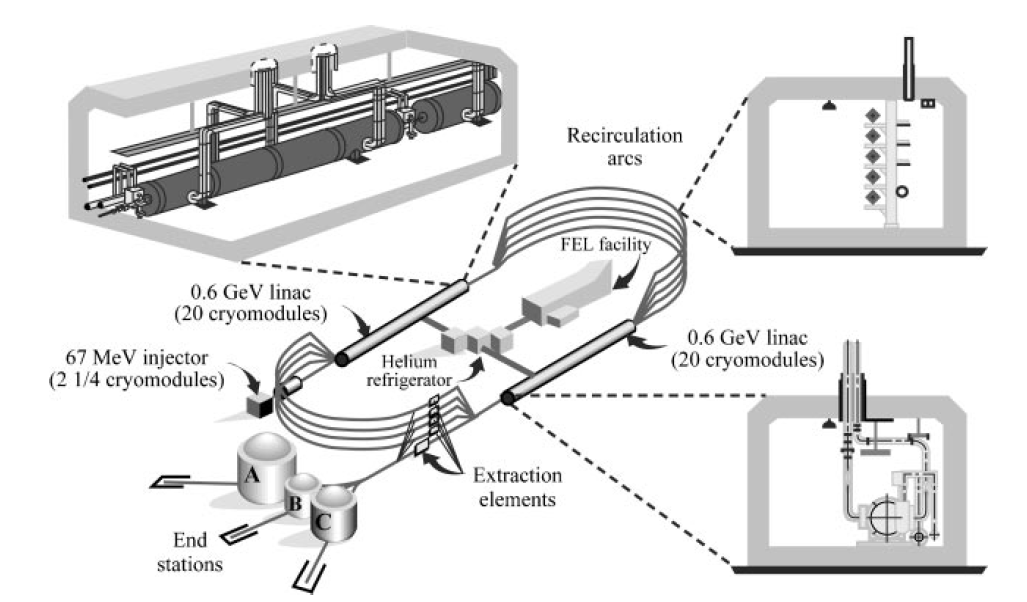
\includegraphics[width=\textwidth]{Pictures/CEBAF.png}
\end{center}
\caption{\label{fig:CEBAF}
Schematic of the accelerator at Jefferson Lab showing the electron source, linear accelerating regions (linacs) and the recirculating arcs. At the time of the \Qs experiment electrons could pass around the accelerator from 1-5 times depending upon the desired energy. Vertical dipole magnets momentum analyze the electrons distributing them in various recirculation arcs at different heights according to the number of passes through the linacs with higher arcs corresponding to lower energy electrons. The three experimental halls A, B and C are also shown.\cite{Leeman}}
\end{figure}

Electron beam polarimetry for \Qs was accomplished using an existing M\o ller polarimeter in Hall C as well as a new Compton polarimeter built specifically for \Q. Polarization values from these were also compared to results from a less accurate Mott polarimeter in the injector region that measures the electron beam polarization at low energies where the Mott scattering cross section is large.

A CAD drawing of the experimental apparatus specific to \Qs installed in Hall C is shown in Figure \ref{fig:QweakApparatus}. This section of the beamline was completely reconstructed to accommodate the \Qs installation including the target, collimators and detector system. The detector system was housed in a concrete hut to further shield from unwanted backgrounds. 



\begin{figure}[!hhhbb]
\begin{center}
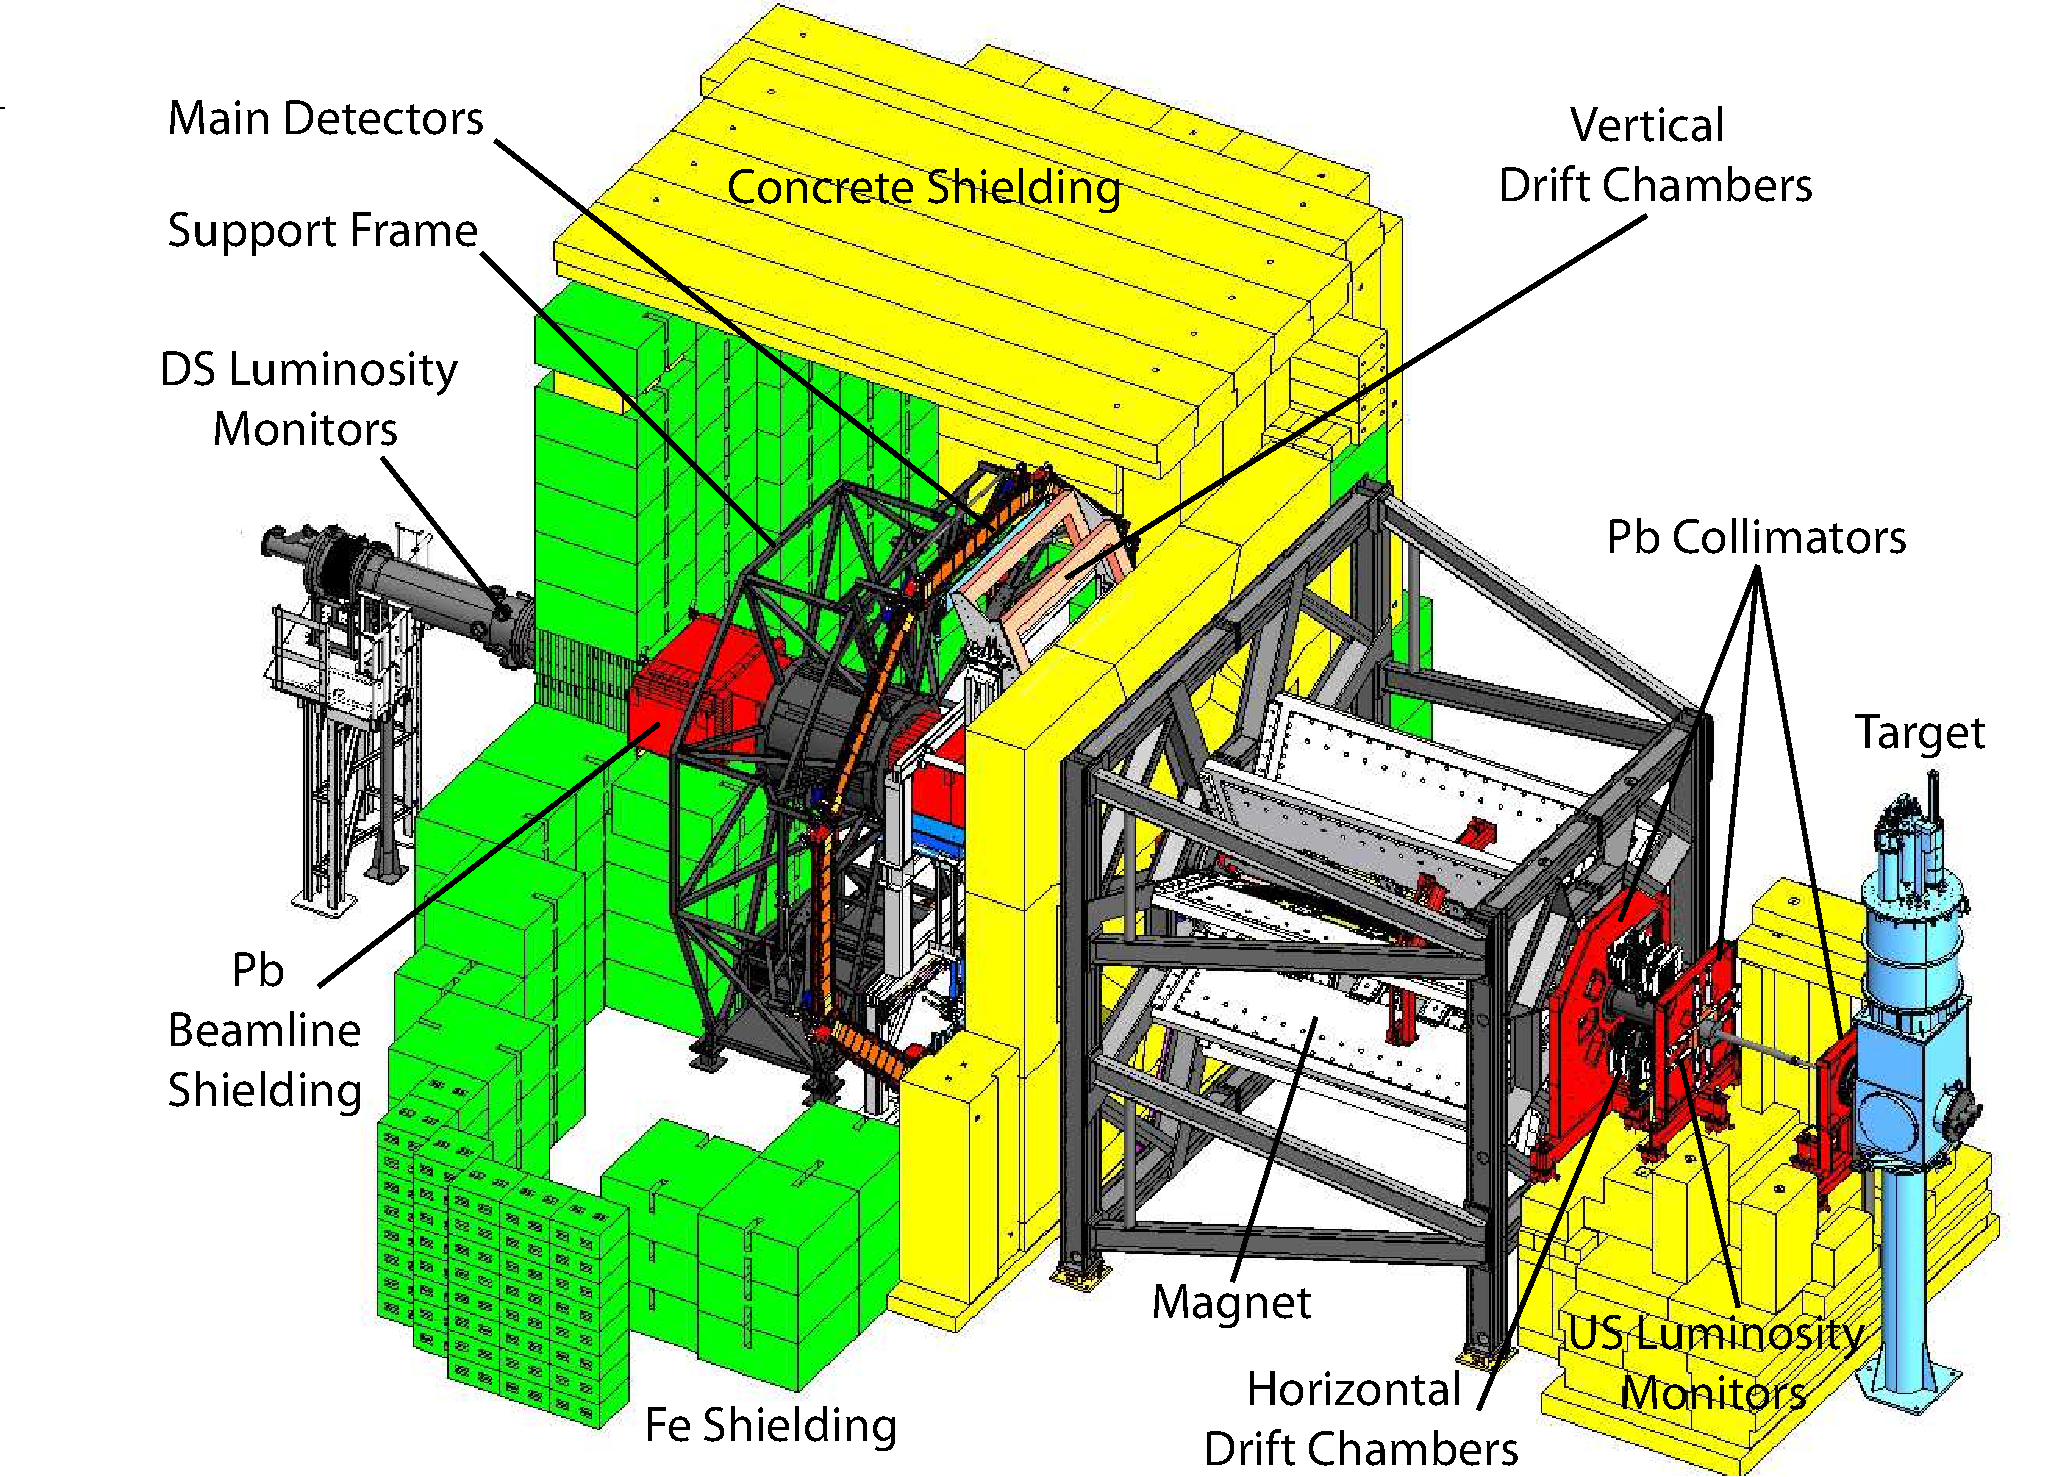
\includegraphics[width=\textwidth]{Pictures/QweakCAD_layout.pdf}
\end{center}
\caption{\label{fig:QweakApparatus}
  CAD drawing of the main \Qs experimental apparatus. The electron beam is incident from the right. The main high current elements shown include the target, torriodal spectrometer, the octogonal array of quartz \v{C}erenkov detectors and the collimator and shielding systems.  Vertical drift chambers directly in front of the detector bars and horizontal drift chambers between the target and spectrometer were used to reconstruct individual tracks during low current running. 
}
\end{figure}

The target was a 34.4~cm liquid hydrogen (\LH) target with thin windows made of aluminum alloy. The \LHs was kept near 20~K with a heat exchanger supplied with liquid helium. A lead collimator selected scattered electrons in a range of angles from 5.8$^{\circ}$ to  11.6$^{\circ}$ in the low $Q^2$ region centered on 0.025~(GeV/c)$^2$ where hadronic effects are relatively insignificant. A series of three lead collimators were used to remove inelastic events upstream of the spectrometer. A torroidal spectrometer (\qtor) was used to focus elastic events onto the detector bars while keeping most of the inelastic events well out of the detector acceptance.

Drift chambers upstream of the spectrometer and directly in front of the main detector bars were used to reconstruct individual event trajectories for the determination of the average experimental $Q^2$. These were operated in extremely low current conditions (50~pA) so that individual events could be resolved. 

Beam position was monitored by a series of beam position monitors (BPM's) located every few meters along the beamline. A fast feedback system (FFB) reading from BPM's in the arc leading to Hall C  was used to stabilize beam energy as well as position and angle at the target.  

Luminosity monitors were placed at two locations downstream from the target near the beam pipe to monitor low angle scattering events such as might be produced by beam halo interacting with small apertures in the beam pipe and M\o ller scattering in the target. Detectors placed in various locations inside the shielded detector region outside the main detector acceptance were used to monitor unwanted backgrounds. 

Greater detail about the subsystems is presented in the sections ahead with emphasis placed upon both the procedures followed and the instrumentation utilized to minimize the uncertainty for \Q.

\section{\label{sctn:electron_source}Polarized Electron Source and Injector}
The program of increasingly sensitive parity-violation experiments at Jefferson Lab over the past decade, including G0, the HAPPEX experiments, PREX, PVDIS and finally Qweak, has created a focus on delivery of the highest quality electron beam with particular attention on the electron source. The electron beam is created by optically pumping a strained superlattice GaAs photo-cathode. The helicity of the laser is transferred to the electrons and the theoretical limit of 50\% polarization attainable with a simple GaAs photo-cathode is exceeded by introducing alternating layers of GaAs with lattice mismatched InGaAs to generate a strained superlattice\cite{Pierce1975}\cite{Maruyama}. Polarizations exceeding 88\% were routinely achieved during \Q.

\begin{figure}[!hbtbhbtb]
\centerline
{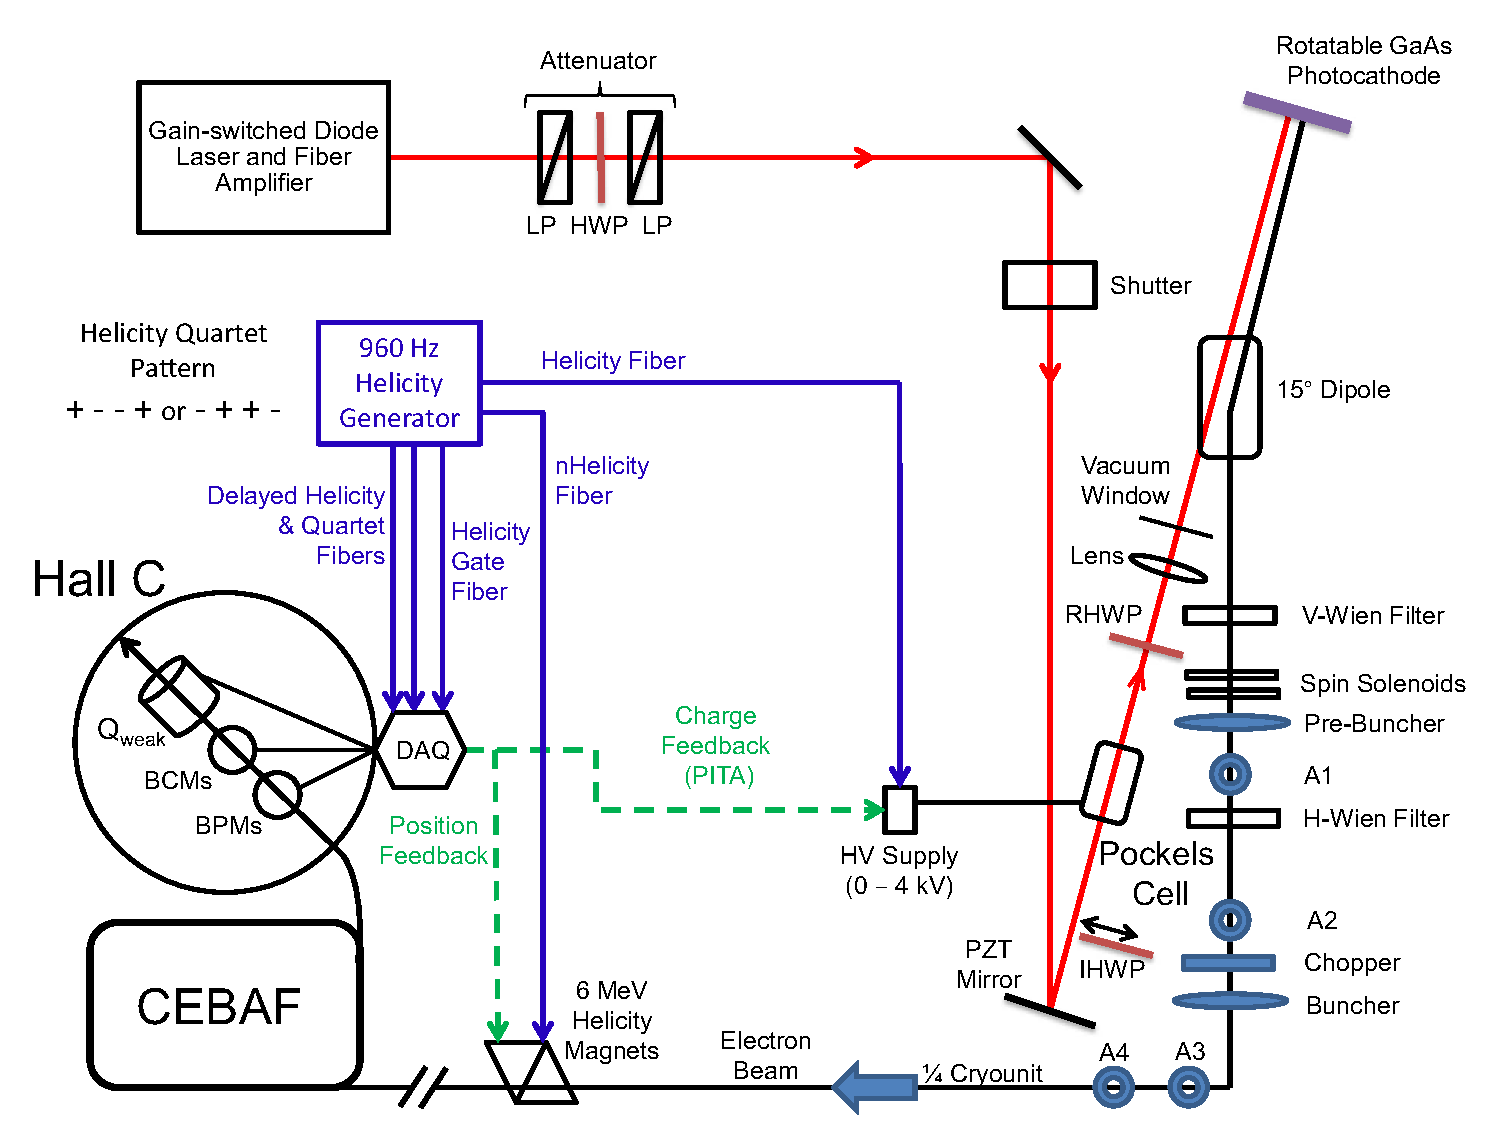
\includegraphics[width=\textwidth,angle=0]{Pictures/jlab_source.pdf}}
\caption{\label{fig:sourcetable} A schematic of the polarized source and injector components used for the \Qs experiment. An IR laser is circularly polarized using a linear polarizer (not shown) followed by a Pockels cell. An optical helicity signal at 960~Hz is used to switch the high voltage on the Pockels cell thus changing the laser helicity. Most of the electrons released from the GaAs photo-cathode by photo-emission carry the same helicity as the laser. A rotatable half-wave plate (RHWP) is used to rotate residual linear polarization to cancel polarization-analyzing gradients on the photo-cathode and polarization gradients across the laser spot.}
\end{figure}

\begin{figure}[ht]
\begin{center} 
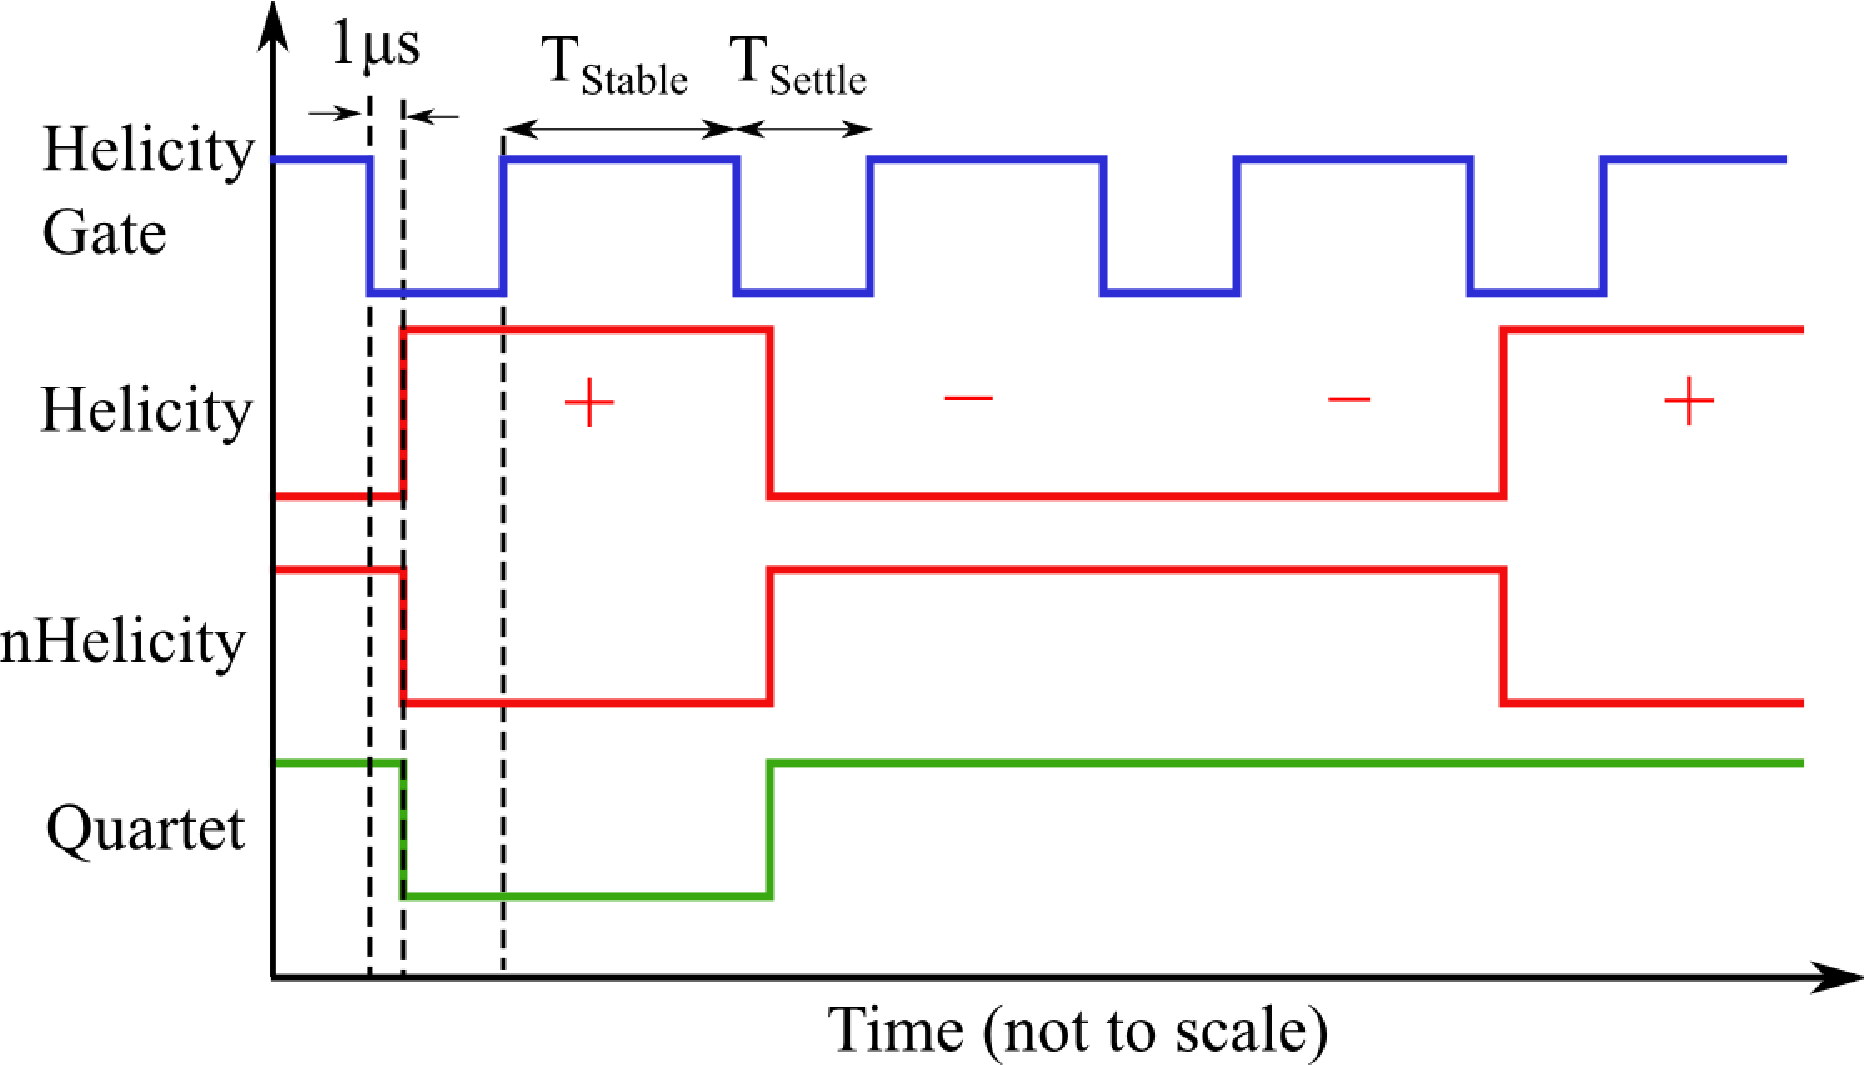
\includegraphics[width=0.7\textwidth]{Pictures/hel_mps_qrt_det_signal_NIM.pdf}
\caption{ \label{fig:helicity_timing} 
Diagram illustrating timing of the helicity signals for the polarized source. The helicity signal (red) controlled the sign of the high voltage across the Pockels cell and always followed a $+ - - +$ or $- + + -$ pattern with the sign of the first element in each pattern chosen using a pseudo-random number generator. The nHelicity signal, the complement of Helicity, ensured that the timing board always drew the same current no matter which helicity state was being signaled. The Helcity Gate signal (blue) was used for timing data acquisition and was lowered $1~\mu$s before each helicity window and stayed low for time $T_{settle}=70~\mu$s to allow for the finite transition time to a new helicity state. Data acquisition was triggered whenever the Helicity Gate signal was high. Lastly, the Quartet signal (green) was used to mark the beginning of each new quartet pattern. }
\end{center}
\end{figure}

The laser is circularly polarized using a linear polarizer followed by a Pockels cell which utilizes an optically active crystal whose birefringence is proportional to the applied voltage across it. A fast switch is used to reverse the polarity of the high voltage across the Pockels cell and thus to flip the laser helicity. Figure \ref{fig:sourcetable} shows a schematic of the polarized electron source. An insertable half-wave plate before the Pockels cell allows the helicity of the laser to be reversed with respect to the high voltage state across the Pockels cell. This provides a sensitive test of systematic false asymmetries associated with high voltage state so that they can be minimized and/or canceled. 

A specially designed electrical timing board was used to control the helicity flip frequency during \Q. The electronics of this board were carefully isolated from other source and experimental electronics to eliminate contamination of detector signals and to minimize effects such as beam motion induced in the source by electronics cross-talk at the helicity reversal frequency\footnote{This was an issue in the HAPPEX-He experiment\cite{Paschke2007}.}. Four signals were generated by the timing board to control the timing of helicity reversal and to trigger data acquisition (see Figure \ref{fig:helicity_timing} for an explanation of the timing signals). The helicity signal was sent to a high voltage optical switch using LED's attached to fiber-optic cable. Although most previous experiments at Jefferson Lab flipped the helicity at 30~Hz, a much faster flip frequency of 961.015~Hz was chosen for \Qs to reduce the effects of drifts in beam, target and detector properties, requiring a redesigned high voltage switch with a rise/fall time of $\sim60 \mu$s \cite{Adderley2012}. 

Careful attention was given to the alignment and polarization of the source laser to minimize helicity-correlated charge and position differences. Further details about the source of these helicity-correlated beam asymmetries (HCBA's) and methods to reduce their effects can be found in the following reference \cite{Paschke2007} and specifics related to the \Qs experiment in a future thesis \cite{Kargiantoulakis}.

Upon emission from the photo-cathode, the electrons are accelerated by an electrostatic field inside what is called the ``electron gun''. The gun bias voltage was increased for \Qs from 100~keV to 130~keV to create a more compact beam and thus reduce aperture losses in the injector region which are known to create intensity asymmetries \cite{Adderley2012}.

The accelerator RF cavities at Jefferson Lab are tuned to resonate at a frequency of 1497~MHz. Each experimental hall has its own source laser pulsed at 1/3 the accelerator frequency or 499~MHz so that all three halls can receive beam at the same time. An RF separator is frequency tuned to kick each of the bunches off the straight line trajectory through three small holes in a metal plate called the chopper. Figure \ref{fig:sourcetable} shows that the electron beam goes through a pre-buncher before the chopper. The pre-buncher is an accelerating cavity tuned such that the electron bunch spans a zero crossing in the RF standing wave making the two ends of the bunch experience opposite sign fields. This slows the frontmost electrons and accelerates the rearmost electrons creating a tighter bunch. Figure \ref{fig:prebuncher} shows a picture of the chopper with and without the prebuncher and how much cleaner the beam is when the prebuncher is used. The beam passes through another buncher after the chopper to further compact the electron pulses before entering cryogenic accelerating cavities further boosting the electrons to relativistic energies before entering the main accelerator. 
\begin{figure}[ht]
\begin{center} 
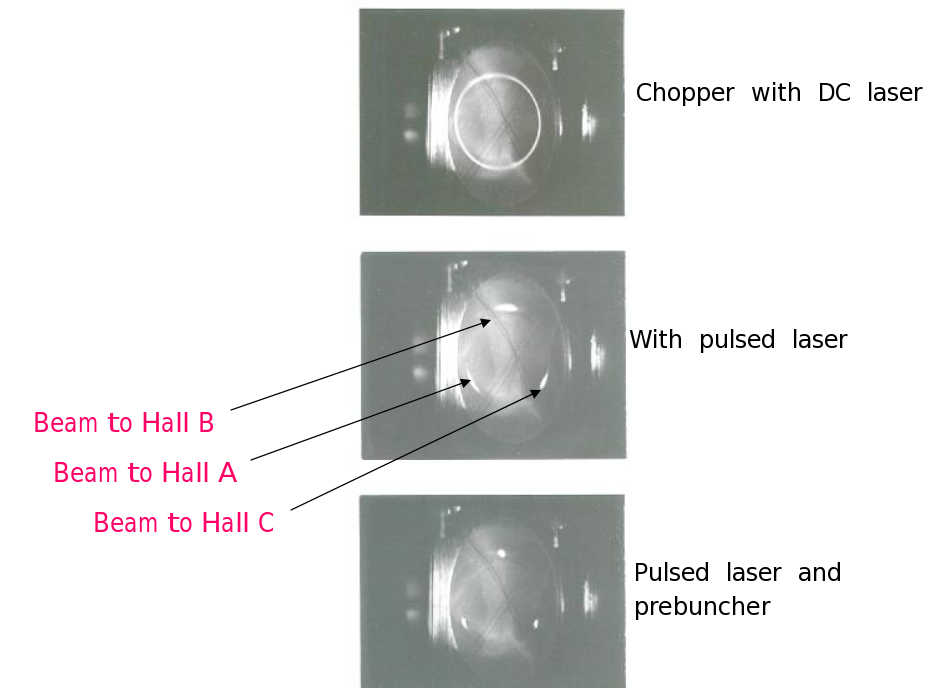
\includegraphics[width=0.7\textwidth]{Pictures/chopper.png}
\caption{ \label{fig:prebuncher} Chopper viewer with beams to three halls shown without pulsed laser, with pulsed laser and with pulsed laser and prebuncher. The small apertures in the chopper disk are not visible in the photograph but are smaller than the spot size in the bottom picture. 
}
\end{center}
\end{figure}
 
Apertures in the source region (labeled A1-A4 in Figure \ref{fig:sourcetable}) are used to clean up the beam. These apertures coupled with helicity-correlated beam position differences can be a significant source of charge asymmetry from differential chopping. 

A double Wien spin-flipper with components labeled as ``H-Wien'', ``V-Wien'' and ``Spin Solenoids'' in Figure \ref{fig:sourcetable}, allows the helicity of the electron beam to be reversed relative to the laser helicity providing another level of diagnostics and cancelation for systematic helicity-correlated differences on the electron beam. A diagram of the double Wien spin-flipper is shown in Figure \ref{fig:double_wien}. The vertical Wien flips the spin from longitudinal to transverse pointing vertically upward. The spin solenoids then serve the dual purpose of focusing the beam and precessing the electron spin clockwise or counterclockwise to make them horizontal and transverse to the direction of propagation. Finally, the horizontal Wien filter rotates the spins in the horizontal plane to any desired angle relative to the direction of propagation such that the spins are properly aligned (typically fully longitudinal) when they enter the experimental hall. Due to inefficiencies associated with setting up the double Wien spin-flipper, during the entire \Qs experiment the spin was reversed only 8 times using the double Wien. A more detailed review of the double Wien filter at Jefferson Lab can be found at \cite{Adderley2011}.
\begin{figure}[ht]
\centering
\framebox{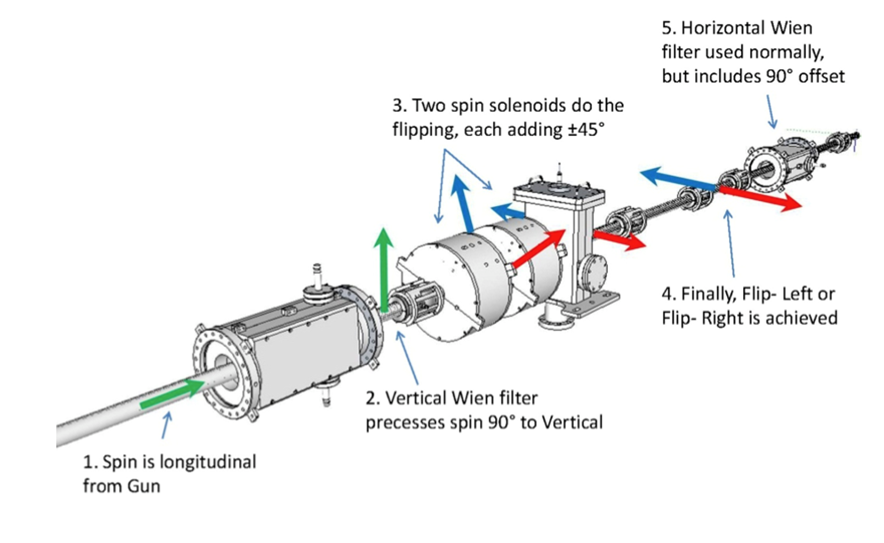
\includegraphics[width=4in]{Pictures/DoubleWien.png}}
\caption{Double Wien filter schematic illustrating the reversal of electron beam helicity.}
\label{fig:double_wien}
\end{figure}

\section{Beam Transport and Monitoring}
\label{sctn:btandm}
As mentioned earlier in this chapter, the accelerator at Jefferson Lab consists of two linacs (north and south) connected by recirculating arcs. Each pass gives an energy of approximately 1.1 GeV to the electrons, allowing certain beam energies to be selected for the experimental halls by choosing the number of passes around the accelerator. The collinear beams for the three halls are extracted at the end of the south linac by an RF extractor that selectively ``kicks'' the beam pulses for the three experimental halls into the direction of their respective beam extraction pipes. A septum magnet further separates the beam trajectories. The beam for Hall C then travels through an arc (to the left looking downstream) before entering the experimental hall. 
\begin{figure}[ht]
\centering
\framebox{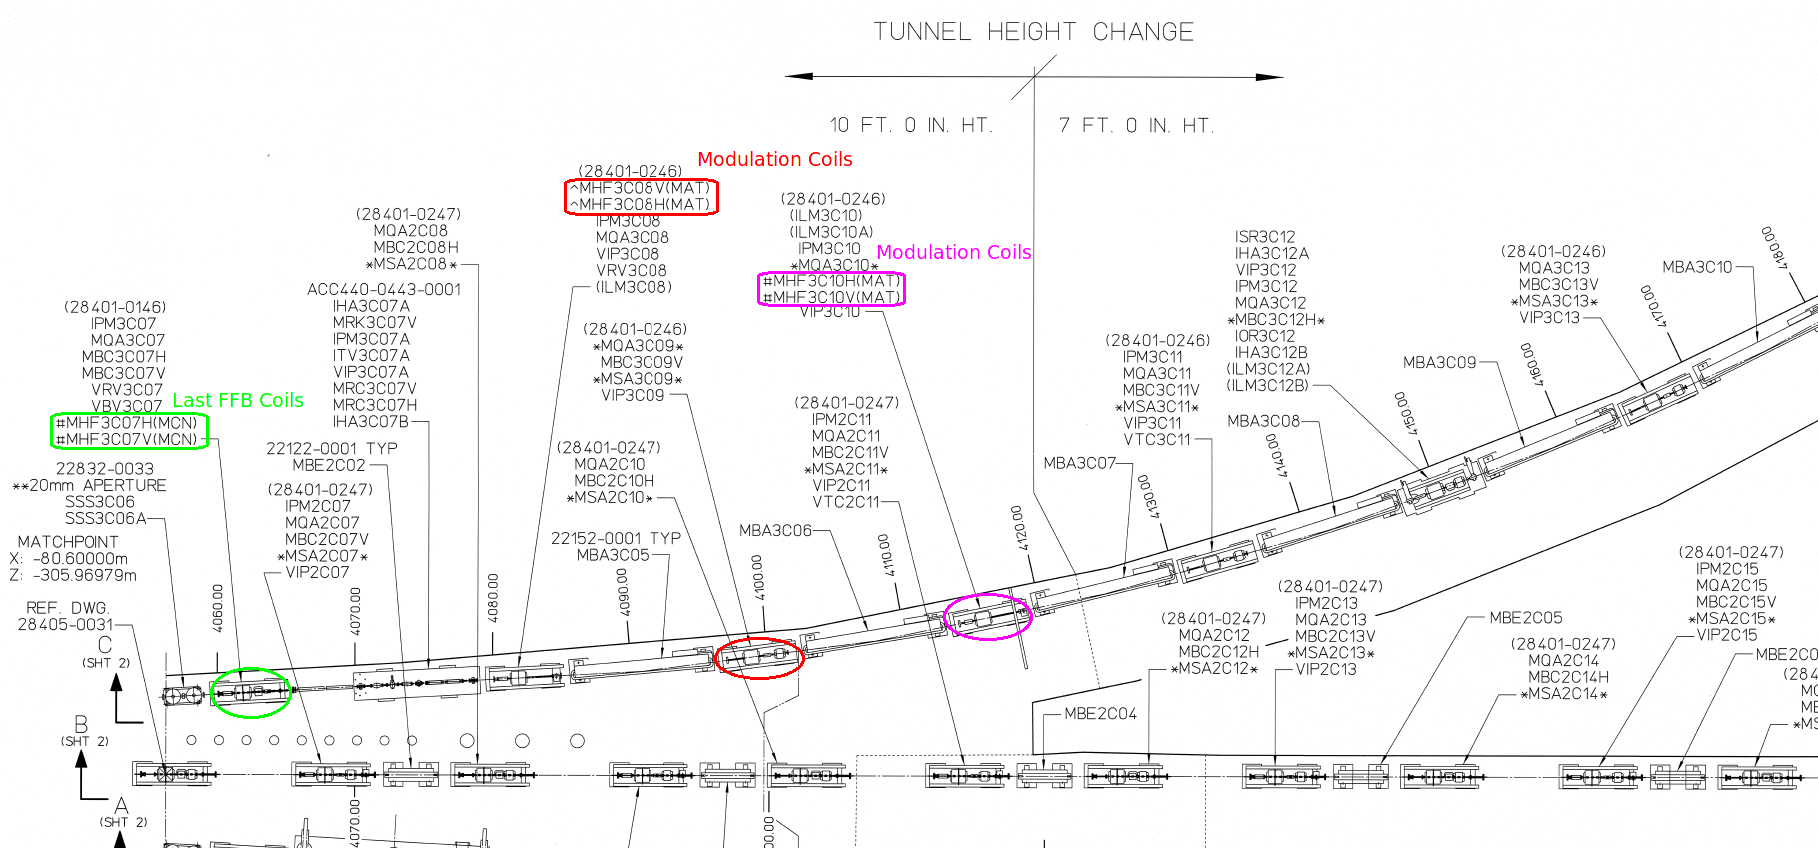
\includegraphics[width=0.99\textwidth]{Pictures/ArcSongSheet.png}}
\caption{Partial engineering diagram of beamline arc heading into experimental Hall C. The most downstream set of fast feedback air-coil corrector magnets and the modulation coils are specifically labeled.}
\label{fig:HallC_arc}
\end{figure}

The position of the electron beam is measured every few meters by beam position monitors (BPM's), which are metal canisters outfitted with four small RF antennae \cite{Barry1991}\cite{Powers1997}. A passing electron bunch creates signals in each antenna proportional to its distance from the antenna allowing the beam position to be measured relative the center of the canister. The signals are amplified, conditioned and averaged before the positions are calculated. Figure \ref{fig:bpm_attennae} shows an illustration of the BPM canister and antennae along with a picture of an installed BPM. BPM's at Jefferson Lab are typically installed such that the antennae are rotated $45^{\circ}$ relative to the horizontal and vertical planes to keep them out of direct line of synchrotron radiation on horizontal and vertical bends. The signals are then rotated in software to give true X and Y positions. The position in the rotated (primed) coordinate system can be calculated as \cite{Geoffrey1993}
\begin{equation}
X'=k\frac{(X^+-X_{off}^+)-\alpha_X(X^--X_{off}^-)}{(X^+-X_{off}^+)+\alpha_X(X^--X_{off}^-)},
\label{eq:x_prime}
\end{equation}
and
\begin{equation}
Y'=k\frac{(Y^+-Y_{off}^+)-\alpha_Y(Y^--Y_{off}^-)}{(Y^+-Y_{off}^+)+\alpha_Y(Y^--Y_{off}^-)},
\label{eq:y_prime}
\end{equation}
where $X^+$, $X^-$, $Y^+$, $Y^-$ are the signals from 4 antennae, $X_{off}^+$, $X_{off}^-$, $Y_{off}^+$, $Y_{off}^-$ are the antenna signals with no beam and $\alpha_{X(Y)}$ is a factor to account for gain differences between the + and -- antennae in the X' (Y') directions\footnote{The $\alpha$ scale factors are given explicitly as $\alpha_{X(Y)}=\frac{X(Y)_+-X(Y)_{off}^+}{X(Y)_-+X(Y)_{off}^-}$.}. The scale factor k is the sensitivity of the BPM at the accelerator frequency of 1497~MHz and depends upon the size of the canister.

  The readout system uses switched electrode electronics (SEE) so that the same amplifier-detector chain is used to read out the + and -- signals sequentially, greatly reducing sensitivity to differential gain and offset changes between readout channels. The electronics switch between the two wires every 4.2~$\mu s$ and integrate the position signal for a 2.9~$\mu s$ window.
\begin{figure}[ht]
\centering
\framebox{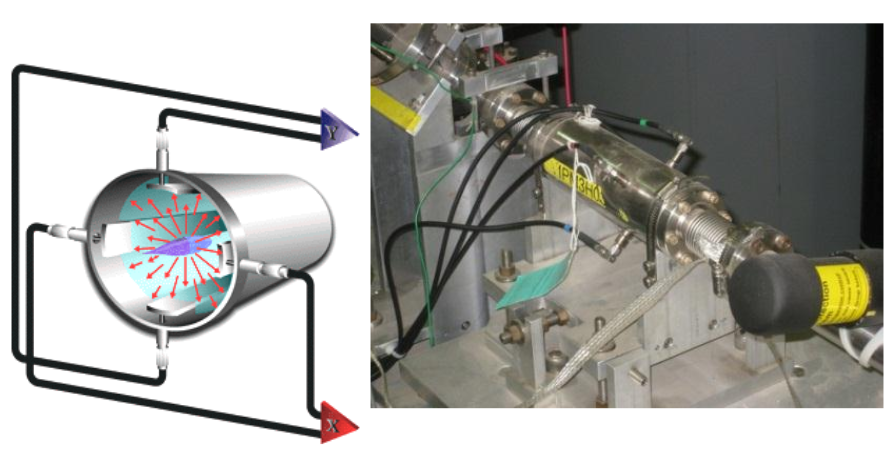
\includegraphics[width=0.99\textwidth]{Pictures/bpm_antennae.png}}
\caption{Left graphic illustrates stripline beam position monitor with four antennae. Position is calculated using the difference of the wire signals in a given direction. Picture on the right shows an actual BPM installed on the beamline. The antenna connections can be seen with cables going to readout electronics.}
\label{fig:bpm_attennae}
\end{figure}

The quoted resolution of the SEE BPM's has been $<100~\mu m$ from $1-1000~\mu A$ \cite{Powers1997}. A study of BPM resolutions in Hall C during the \Qs experiment, independently measured the resolution of the SEE BPM's as well as the dependence of this resolution on current. Under the assumption that all similar BPM's have the same intrinsic resolution, she used pairs of BPM's in a drift region of the Hall C beamline to predict the position of a third BPM and determined that the resolution of a single BPM at $180~\mu A$ is $\sim 0.9~\mu$m for each MPS which is about 1~ms ( see \cite{Waidyawansa} appendix A).

Superharps located at key positions along the beamline are used to measure the beam profile and absolute position. These consist of a motor-actuated triplet of thin wires ($22~\mu m$ diameter) at fixed angles relative to each other (two wires perpendicular to each other and a third wire in the same plane at 45$^{\circ}$ to the other two wires) which are passed through low current beam. The electrical signals generated in the wires as they pass through the beam are used to reconstruct the beam profile \cite{Yan1995}. Superharps are used to verify that the beam size and profile agree to within tolerance with the beam optics model. For example, having a beam spot size much smaller than the laser profile is critical in the region of the Compton polarimeter where the laser interacts with the electron beam. A superharp in the Compton region was used to verify that the beam spot size was close to the specified $1\sigma$ radius of $40~\mu$m. Superharps were also used to determine the shape of the beam and to check for the presence of asymmetric or unusual beam halo.

Superharps also serve a critical function in measuring the electron beam energy. The absolute beam position and angle is measured at three locations, upstream, at the center and downstream of the Hall C arc using pairs of superharps. The fields of dipole bending magnets in the arc have been mapped to good precision using a combination of Hall and NMR probes and all higher order magnets (sextapoles and quadrupoles) have their field integral set to zero. In this configuration, the beam dispersion at the center of the Hall C arc is large (12~cm/\%). The beam momentum can be calculated as 
\[
p=\frac{e}{\theta}\int B~dl,
\]
where $\theta$ is the net bend angle of the beam and $\int B~dl$ is the total magnetic field integral. The beam energy can then be obtained from $p$ with simple relativistic kinematics.

Differential changes in beam energy are monitored using BPM's located in the Hall~C arc. Higher order optical beamline elements (sextapoles and quadrupoles) create a dispersion in the arc which depends on beam tune. A typical tune for \Qs was around 4~cm/\% at the point of highest dispersion in the arc. The BPM located at this position of highest dispersion is called BPM3c12 and the horizontal beam position at this location, given by BPM3c12X, was used by \Qs as a relative energy monitor. 

A set of 4 air-coil dipole magnets (2 horizontal and 2 vertical) in the Hall C arc are used as part of a feedback system to remove beam position and angle motion at the target. This feedback system called ``Fast Feedback'' (FFB) utilizes BPM's in the Hall C arc and tunnel upstream of the experimental hall to determine frequency components of the beam's motion and drives the FFB dipole coils to null those frequencies. The most downstream set of FFB coils is labeled in Figure \ref{fig:HallC_arc}. The system is specifically tuned to null frequencies that are harmonics of the 60~Hz line noise \cite{Lebedev}. Because the accelerator mixes position and angle with beam energy, the FFB system also includes a BPM in the highly dispersive region of the Hall C arc as a relative energy measurement. Energy fluctuations are corrected by feeding back on a Vernier on one of the accelerating cavities in the south linac. This system was active throughout the \Qs experiment.

A second set of 4 air coil dipole magnets (2 horizontal and 2 vertical) in the Hall C arc were used to intentionally drive the beam in position and angle so that the sensitivity of the main detector to these parameters could be measured. The intentional driving of the beam for calibration of the main detector sensitivities is referred to as ``beam modulation''. The beam modulation  coils are labeled in Figure \ref{fig:HallC_arc}. In addition to these air coil magnets, the beam modulation system also utilized a Vernier on one of the south linac accelerating cavities for intentional modulation of energy. The use of the beam modulation system to calibrate the detector responses to beam energy, position and angle and to correct the main detector to remove these sensitivities is dealt with in detail in Chapters \ref{Chapter4} and \ref{Ch:BMod_correction}.

Beam intensity or current was measured during the \Qs experiment using six beam current monitors (BCM's) upstream of the target, although not all six were available for the entire experiment. The BCM's are cylindrical, stainless steel microwave cavities tuned to resonate at the accelerator frequency (1497~MHz). The $TM_{010}$ mode of the BCM's is proportional to beam current but insensitive to electron bunch length and position \cite{Denard2001}. The BCM's were enclosed in a temperature stabilized box to preserve their resonance tune. The BCM's were calibrated using a parametric current transducer (PCT), often referred to as the ``Unser''. Although the Unser provides a highly accurate current reading, it is subject to slow drifts which compromise its usefulness as a continuous monitor.

In Run 1 of the \Qs experiment, a pair of BCM's (BCM1 and BCM2) were used to normalize the main detector signals to charge. In Run 2 a new set of BCM's were used with updated digital electronics which increased the resolution of the beam current measurements. One method for determining BCM resolution involves taking the difference in the asymmetries measured in two BCM's located close to each other on the beamline. This difference between the two BCM's is termed the ``double difference'' since it is a difference between two measurements of asymmetry between states of opposite helicity. Since both BCM's are expected to be measuring exactly the same beam and have approximately the same intrinsic resolution, the width of the double difference distribution is $\sqrt{2}$ times the BCM resolution. Figure \ref{fig:BCM_dd_width} shows the double difference using BCM's 1 and 2 which were used in Run 1 and the double difference using BCM's 7 and 8 outfitted with new electronics.

\begin{figure}[ht]
\centering
\framebox{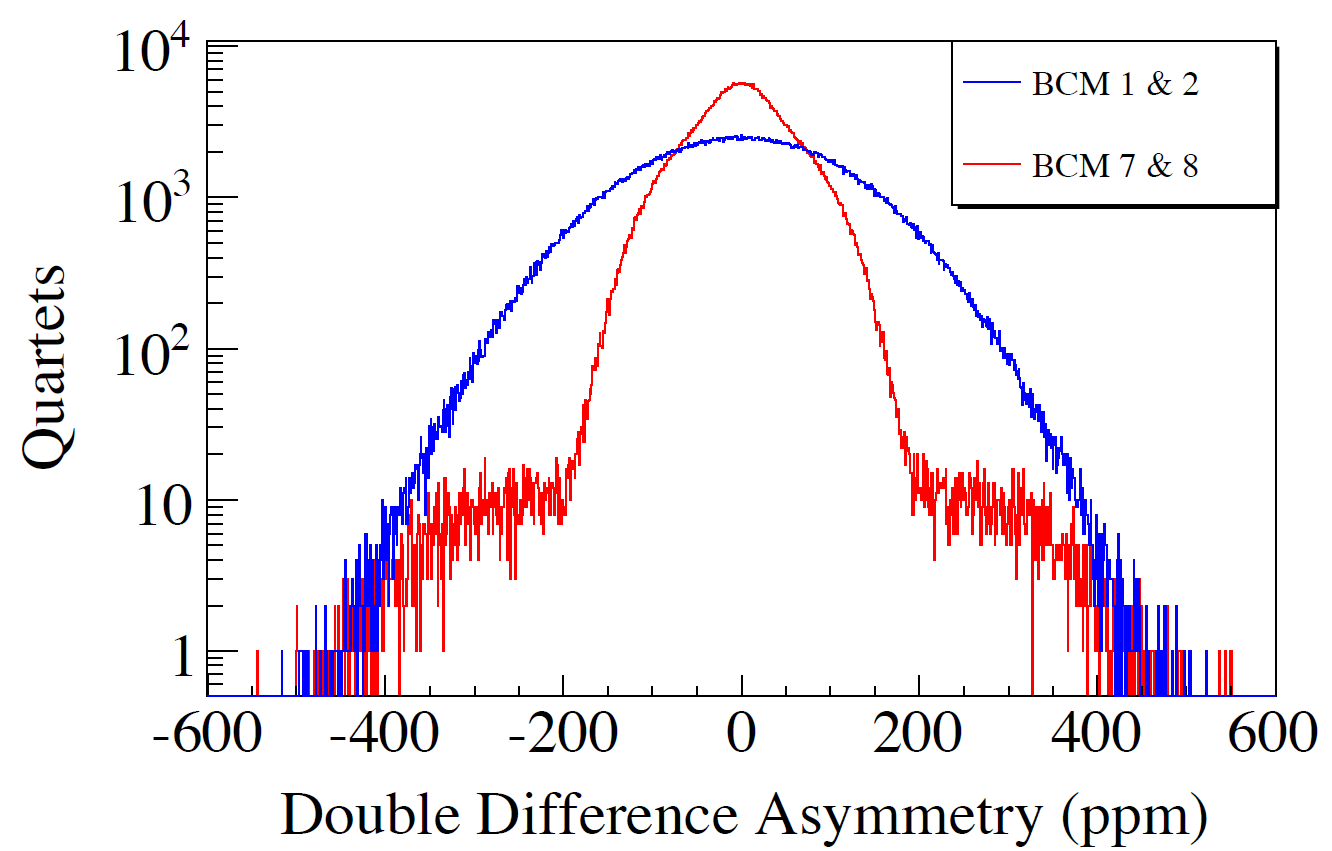
\includegraphics[width=3in]{Pictures/BCM_dd.png}}
\caption{Charge asymmetry double difference (DD) plots (typical 1 hour run) for two pairs of BCM's used in the \Qs experiment. Double difference plots show half the difference in signal between two BCM's measuring the same beam current and as such they are a measurement of the intrinsic BCM noise. BCM's 1 and 2 (blue) have an RMS DD width of 115~ppm while BCM's 7 and 8 (red) have an RMS DD width of 57~ppm.}
\label{fig:BCM_dd_width}
\end{figure}

\section{Polarimetry}
Electron beam polarization enters as a multiplicative factor in determining the parity-violating asymmetry from the measured raw asymmetry (Equation \ref{eq:raw_asymmetry}), requiring a heavy emphasis on polarimetry for \Q. Electron beam polarization was determined for \Qs using the existing M\o ller polarimeter as well as a new Compton polarimeter installed specifically to meet the demands of \Q. Although the M\o ller polarimeter can measure beam polarization to $<1\%$ within a few hours, it is limited to low currents $\sim 1~\mu$A and it is invasive, requiring hours each week of dedicated beam time. The Compton polarimeter can provide continuous, non-invasive polarization measurements at the current of the experiment. The operation of the two polarimeters as well as the results of each are discussed below.

\subsection{M\o ller Polarimeter}
Quantum electrodynamics (QED) accurately predicts a spin dependence in the cross section  of polarized M\o ller (electron-electron) scattering. The spin-dependent cross section for longitudinally polarized, ultra-relativistic electrons can be written at tree level as \cite{Hauger2001}
\begin{equation}
\frac{d\sigma}{d\Omega^{cm}}=\frac{d\sigma_0}{d\Omega^{cm}}\left(1+P_t^{||}P_b^{||}A_{zz}(\theta )\right),
\end{equation}
where the unpolarized cross section at high energy is given by \[\frac{d\sigma_0}{d\Omega^{cm}}=\left(\alpha(4-\sin^2\theta)/2m_e\gamma\sin^2\theta\right)^2,\]  and $P_{t(b)}^{||}$ is the longitudinal polarization of the target (beam). $A_{zz}$, the maximum scattering asymmetry as a function of angle is given by the following expression:\[A_{zz}(\theta )=-\sin^2\theta(8-\sin^2\theta )/(4-\sin^2\theta )^2.\] If the target polarization is known\footnote{Since only the two valence electrons of the 26 in iron are polarizable, the maximum effective target polarization $P_t$ is $\sim$8\%. A potentially significant uncertainty arising from Fermi motion of inner atomic electrons, was first described by Levchuk \cite{Levchuk1994}. The Hall C M\o ller was designed with a large acceptance to make this effect small enough to correct for it with a small uncertainty.}, the electron beam polarization can be obtained from the measured scattering asymmetry between beam polarization states of right and left helicities which is given as 
\begin{equation}
A_{M\o ller}=\frac{\frac{d\sigma}{d\Omega^{cm}}^{\uparrow\uparrow}-\frac{d\sigma}{d\Omega^{cm}}^{\downarrow\uparrow}}{\frac{d\sigma}{d\Omega^{cm}}^{\uparrow\uparrow}+\frac{d\sigma}{d\Omega^{cm}}^{\downarrow\uparrow}}=A_{zz}P_b^{||}P_t^{||},
\label{eq:moller_asym}
\end{equation}
where $\alpha$ is the fine structure constant, $\frac{d\sigma}{d\Omega^{cm}}^{\downarrow\uparrow}$ is the differential scattering cross section for target and beam spins aligned and $\frac{d\sigma}{d\Omega^{cm}}^{\uparrow\uparrow}$ is for the beam and target spins anti-aligned. In practice, $A_{M\o ller}$ is measured as the difference in the numbers of scattered electrons between the two helicity states. The kinematics of the M\o ller polarimeter in Hall C are set to select the maximum analyzing power with the center of mass scattering angle of $\theta_{cm}=90^{\circ}$ giving $A_{zz}\approx-\frac{7}{9}$. 

The target for the Hall C M\o ller is a thin iron foil placed directly in the electron beam and polarized to the point of saturation in the direction of the electron momentum using a superconducting 3.5~T magnet.  Both the scattered electron and the dislocated atomic electron are detected in coincidence by symmetric detectors on both sides of the electron beam. A tight timing cut on the coincidence highly suppresses backgrounds primarily from Mott scattering. Two quadrupole magnets momentum analyze the scattered electrons so that the desired events are selected and the majority of background events blocked by a system of collimators. A diagram of the M\o ller polarimeter is shown in Figure \ref{fig:Moller_diagram}. The difference in the number of coincidences between right and left beam helicity states divided by the total number for both states gives the asymmetry $A_{M\o ller}$.

\begin{figure}[ht]
\centering
\framebox{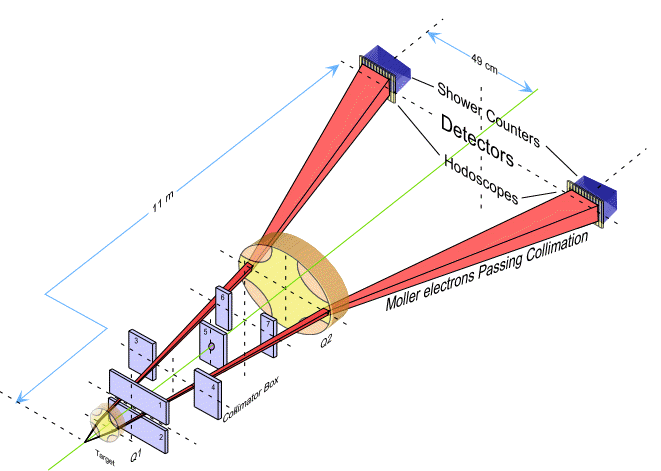
\includegraphics[width=4in]{Pictures/moller_diagram.png}}
\caption{Diagram showing key components of the Hall C M\o ller polarimeter. }
\label{fig:Moller_diagram}
\end{figure}

During \Qs the beam polarization was measured using the M\o ller 2-3 times per week. Beam current during these measurements was around $1~\mu$ A to keep uncertainty from target depolarization low. The list of systematic uncertainties associated with the M\o ller measurements is given in Table \ref{tab:moller_systematics}. During Run 1 an additional systematic uncertainty of 0.89\% was included to account for an intermittent short in one of the M\o ller quadrupoles which altered the analyzing power $A_{zz}$. 

\begin{table}[!h]
  \centering
    \begin{tabular}{|l|c|c|} \hline
                           & Uncer- & $dA/A$ \\ 
      Source & tainty & (\%) \\ \hline
      Beam position $X$     & 0.5 mm      & 0.17     \\
      Beam position $Y$     & 0.5 mm      & 0.28     \\
      Beam direction $X^\prime$    & 0.5 mrad    & 0.1      \\
      Beam direction $Y^\prime$    & 0.5 mrad    & 0.1      \\
      Q1 current                 & 2\%         & 0.07     \\
      Q3 current                 & 3\%         & 0.05     \\
      Q3 position                & 1 mm        & 0.01     \\
      Multiple scattering        & 10\%        & 0.01     \\
      Levchuk effect             & 10\%        & 0.33     \\
      Collimator position        & 0.5 mm      & 0.03     \\
      Target temperature         & 100\%       & 0.14     \\
      B-field direction          & 2$^\circ$   & 0.14     \\
      B-field strength           & 5\%         & 0.03     \\
      Spin depolarization        & --~         & 0.25     \\
      Electronic dead time       & 100\%       & 0.05     \\
      Solenoid focusing          & 100\%       & 0.21     \\
      Solenoid position($X,Y$)     & 0.5 mm       & 0.23     \\
      High current extrap. & --~         & 0.5      \\
      Monte Carlo statistics     & --~         & 0.14     \\ \hline
      ~                          & Total       & 0.83     \\ \hline
    \end{tabular}
  \caption{{Table of uncertainties for the Hall C M\o ller polarimeter for Run 2 of the experiment taken from the \Qs instrumentation paper \cite{QweakNIM}. During Run 1 an intermittent short in one of the polarimeter quadrupoles added an uncertainty not included here.}}
  \label{tab:moller_systematics}
\end{table}

\subsection{\label{sctn:compton}Compton Polarimeter} 
Compton polarimetry relies on electron-photon (e$\gamma$) scattering to determine electron beam polarization. A circularly polarized laser beam of photons intersects the electron beam at a small crossing angle. The e$\gamma$ cross section is small enough that its affect on the electron beam can be neglected; however, the cross section depends slightly upon the relative helicities of the electron and photon. The tree level spin-dependent cross section of longitudinally polarized electrons on circularly polarized photons with collinear (opposite direction) momenta\footnote{A zero angle crossing of the laser and electron beam is assumed. The Hall C Compton crossing angle is $1.33^{\circ}$ or $23.2~mrad$. The correction to account for the non-zero crossing angle is negligible for the kinematics of the Compton polarimeter. \cite{Denner1999}} is given by QED as \cite{Prescott1973}\cite{Tolhoek1956}
\begin{equation}
\frac{d\sigma}{d\rho}=\frac{d\sigma_0}{d\rho} \mp P_eP_{\gamma}\cos\theta\frac{d\sigma_1}{d\rho},
\label{eq:compton_cx}
\end{equation}
where $\frac{d\sigma_0}{d\rho}$ is the unpolarized cross section, $\frac{d\sigma_1}{d\rho}$ is the longitudinal spin-dependent piece of the cross section, $P_{e(\gamma)}$ is the electron (photon) polarization and $\theta$ is the angle between the electron spin and its momentum. The -- sign of the second term corresponds to the photon whose helicity is parallel to its momentum (opposite the electron momentum)\cite{Prescott1973}. The two components of the cross section can be shown to be
\begin{equation}
\frac{d\sigma_0}{d\rho}=2\pi r_0^2a\left[\frac{\rho^2(1-a)^2}{1-\rho(1-a)}+1+\left(\frac{1-\rho(1+a)}{1-\rho(1-a)}\right)^2\right],
\label{eq:unpol_compton_cx}
\end{equation}
and 
\begin{equation}
\frac{d\sigma_1}{d\rho}=2\pi r_0^2a\left[\left(1-\rho (1+a)\right)\left(1-\frac{1}{1-\rho(1-a)}\right)^2\right],
\label{eq:spin_dep_compton_cx}
\end{equation}
where $r_0$ is the classical electron radius, $\rho=k'/k_{max}$ is the ratio of the scattered photon energy to the maximum scattered photon energy in the lab frame and $a=1+4kE/m_e^2$ is a kinematic factor where $k$ is the incident photon energy and $E$ is the incident electron energy measured in the lab frame. The asymmetry then comes from the longitudinal spin dependent term of Equation \ref{eq:spin_dep_compton_cx} and takes the form
\begin{equation}
A_{l}=\frac{\frac{d\sigma}{d\Omega^{cm}}^{\uparrow\uparrow}-\frac{d\sigma}{d\Omega^{cm}}^{\downarrow\uparrow}}{\frac{d\sigma}{d\Omega^{cm}}^{\uparrow\uparrow}+\frac{d\sigma}{d\Omega^{cm}}^{\downarrow\uparrow}}=\frac{d\sigma_1}{d\rho}/\frac{d\sigma_0}{d\rho},
\label{eq:compton_asym}
\end{equation}
where the subscript $l$ emphasizes that this is only for longitudinal electron polarization.
Thus, if the photon polarization is known, the electron beam polarization can be determined from the measured asymmetry using the following relationship:
\begin{equation}
A_{measured}=P_eP_{\gamma}A_{Compton}\Longrightarrow P_e=\frac{1}{P_{\gamma}}\left(\frac{A_{measured}}{A_{l}}\right).
\label{eq:compton_pol}
\end{equation}
Plots of the unpolarized differential cross section and of the asymmetry $A_l$ as a function of back-scattered photon energy are shown in Figure \ref{fig:compton_cx}. The asymmetry changes sign in the center of the spectrum and reaches a maximum at the kinematic endpoint for maximum back-scattered photon energy.

\begin{figure}[ht]
\centering
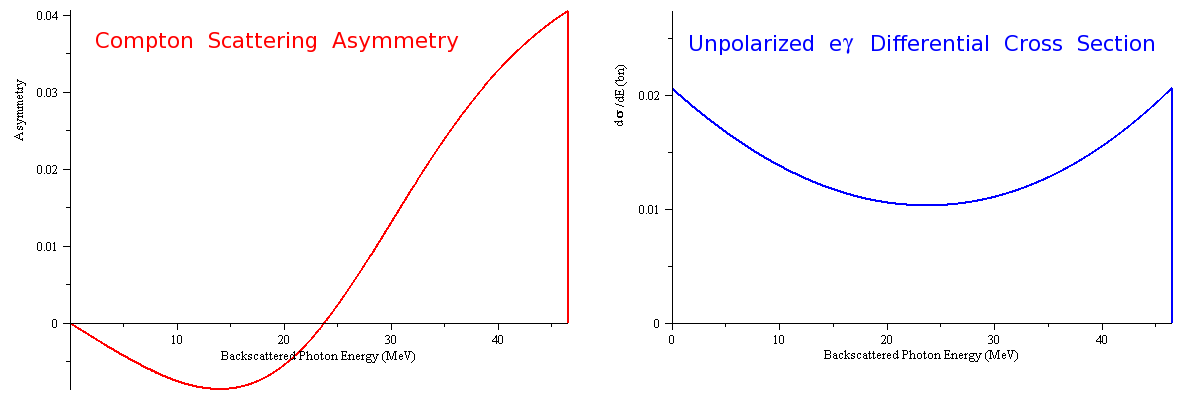
\includegraphics[width=0.99\textwidth]{Pictures/compton_cx.png}
\caption{Compton scattering asymmetry and differential cross section shown at the kinematics of the \Qs experiment using a green (532~nm) laser at 0$^{\circ}$ crossing angle. (Right)Average (unpolarized) differential cross section for electron-photon scattering. (Left) Scattering asymmetry for longitudinally polarized electrons on circularly polarized photons versus back-scattered photon energy. }
\label{fig:compton_cx}
\end{figure}
The Hall C Compton polarimeter was designed to measure the scattering asymmetry for both the back-scattered photons and the Compton scattered electrons. An illustration of the system is shown in Figure \ref{fig:compton_layout}. The electron beam is bent through a chicane by a set of 4 identical dipole magnets. At the center of the chicane the electron beam is 0.57~m lower than its usual trajectory and at this point it intersects a laser-fed Fabry-Perot optical cavity where the Compton interaction occurs. The scattered photons in the full $4\pi$ solid angle in the electron rest frame are contained in a small-angle cone in the lab frame centered on the electron beam trajectory and are captured by the photon detector, a scintillating crystal placed 4.3~m downstream of the Compton interaction point. The electron detector, located 5~mm above the electron beam directly upstream of the fourth dipole, measured the asymmetry versus energy spectrum of the scattered electrons momentum-analyzed by the third dipole of the chicane.
\begin{figure}[ht]
\centering
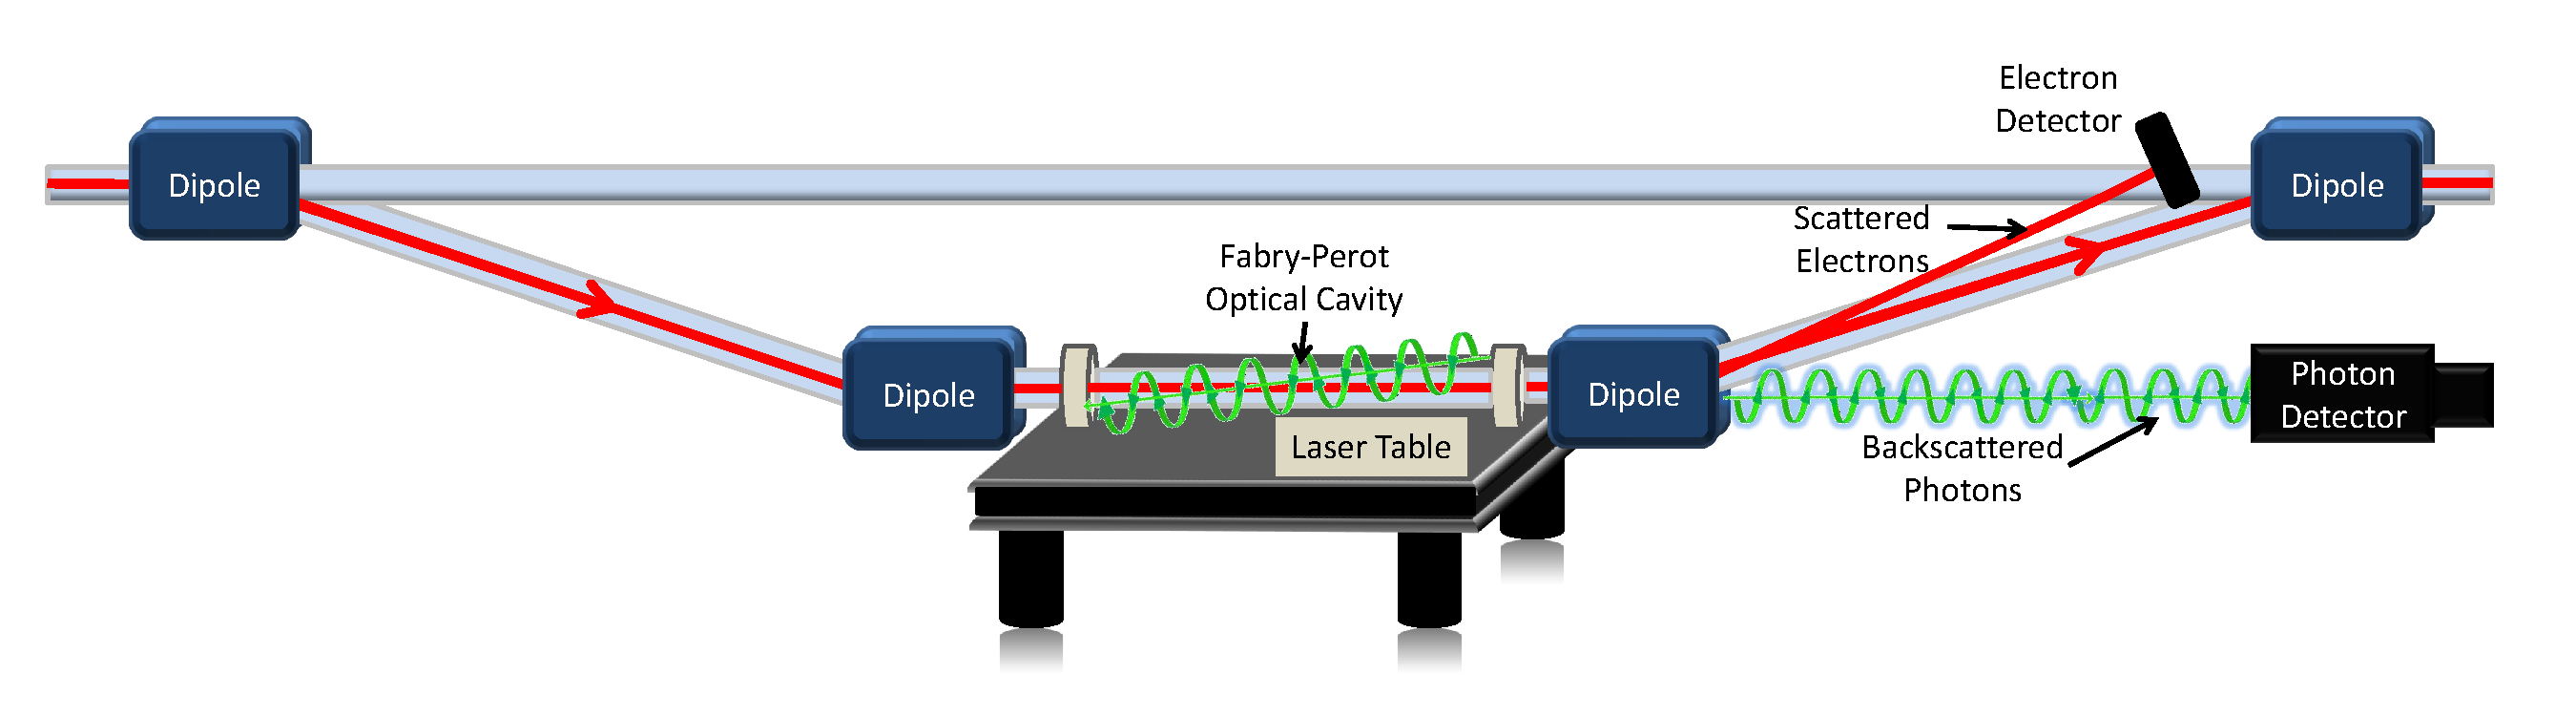
\includegraphics[width=0.99\textwidth]{Pictures/Compton_layout.pdf}
\caption{Illustration of Compton polarimeter showing magnetic chicane, laser table, and electron and photon detectors. }
\label{fig:compton_layout}
\end{figure}
Design and construction of the photon target for the Compton polarimeter was one of the primary concerns of the author early in this experiment. A Coherent Verdi-V10 laser (details on the laser can be found in \cite{Verdi10}) delivered 10~W of green light (532~nm) that was mode-matched to an 84~cm long Fabry-Perot optical cavity. During Run 2 the optical cavity had high-reflectivity mirrors (R=99.5\%) yielding a cavity gain close to 200 with more than 1400-1800~W of stored power depending upon the quality of the mode-matching. Lower reflectivity mirrors used in Run 1 led to more than a factor of 2 reduction in stored power and a poorer signal to background ratio. 

Knowledge of laser polarization inside the optical cavity, housed inside the electron beam vacuum pipe, is essential to the integrity of the electron polarization measurement (see eq. \ref{eq:compton_pol}). A novel method used to determine intracavity laser polarization introduced during Run 2 made this key uncertainty almost negligible. Further details on the setup and analysis for the laser/photon target will be provided in Chapter \ref{Ch:Compton_Laser}.

The photon detector consists of a square matrix of four 20~cm long lead tungstate (PbWO$_4$) scintillating crystals each with a 3~$\times$~3~cm$^2$ cross section attached to a single 7.6~cm Hamamatsu R4885 photo-multiplier tube (PMT) located on the downstream face. The photon detector was maintained at $14^{\circ}$C giving a light yield increase of 20\% relative to the usual $21^{\circ}-24^{\circ}$C temperature of Hall C. The signal from the photon detector was digitized using a flash analog-to-digital converter (FADC) with 200~MHz sampling. The signal was digitally integrated over each MPS and the accumulated sum recorded. In addition to the accumulator sum, a single self-triggered 250-sample waveform of a photon pulse in the detector was digitized and saved for each MPS allowing construction of the detected pulse spectrum for calibration purposes. The laser was continuously cycled on and off for background subtraction in a continuous pattern of 60 seconds on and 30 seconds off. ``Laser off'' means the optical cavity was unlocked and the laser beam blocked. Some periods during the experiment did not have the light blocked and a small residual beam of light leaked into the cavity, necessitating a small correction. Figure \ref{fig:laser_onoff} shows a graph of the photon detector yield (accumulated sums) versus time clearly demonstrating the increase of light yield during laser on periods.
\begin{figure}[ht]
\centering
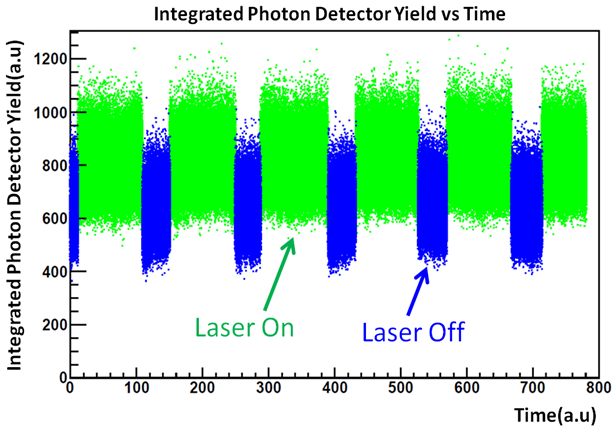
\includegraphics[width=0.6\textwidth]{Pictures/laser_onoff.png}
\caption{Photon detector yield versus time clearly showing the transitions between laser on and off periods.}
\label{fig:laser_onoff}
\end{figure}
Statistical uncertainty for the photon detector measurements remained relatively high throughout \Qs so that its usefulness in tracking polarization between M\o ller polarization measurements was not realized. The analyzing power and non-linearity of the photon detector data were determined by a combination of GEANT4 simulation and direct measurement (for details see \cite{Cornejo}). The combined statistical and systematic errors associated with the photon detector analysis were too large to provide useful polarization values for \Q.

The electron detector is composed of a multiple plane diamond microstrip detector. Each detector plane is a thin ($500~\mu$m thick) 21~cm~$\times$~21~cm diamond wafer. The front surface of each wafer has 96 metal microstrips each $180~\mu$m wide with a $20~\mu$m gap between them, while a single electrode covers the entire back of the wafer. When an electron travels through the diamond it creates a trail of electron-hole pairs. A high voltage applied across the electrodes makes the electron-hole pairs migrate towards opposite plates causing an electrical pulse in the nearest microstrip(s). Pulses are conditioned and summed individually for each strip over each MPS window. Three of four parallel detector planes were used during \Qs with an event trigger requiring a hit in at least two of the three planes. A small set subset of the data was taken requiring a coincidence in three planes which was useful for diagnostic purposes and for calculating dead time.

Two parameters required before beam polarization can be extracted from the asymmetry spectrum are the microstrip-to-energy conversion factor and the strip offset. Only when these are known can the asymmetry versus microstrip spectrum be properly mapped its corresponding energy spectrum. A calculation of the strip/MeV conversion factor was made using a magnetic map of the third dipole in the chicane combined with the measured electron path. A fit procedure for locating the ``Compton edge''\footnote{Compton scattering asymmetry spectra are typically shown versus back-scattered photon energy or electron energy lost to the photon. The ``Compton edge'' is the largest possible energy loss corresponding to the direct $180^{\circ}$ back-scattering of the photon which also corresponds to the electrons which are least energetic. The Compton edge is obvious in Figure \ref{fig:compton_cx} since no Compton scattering occurs at higher energies.} gave the necessary offset allowing the Compton asymmetry spectrum to be fit with only one additional parameter, the electron polarization.
\begin{figure}[ht]
\centering
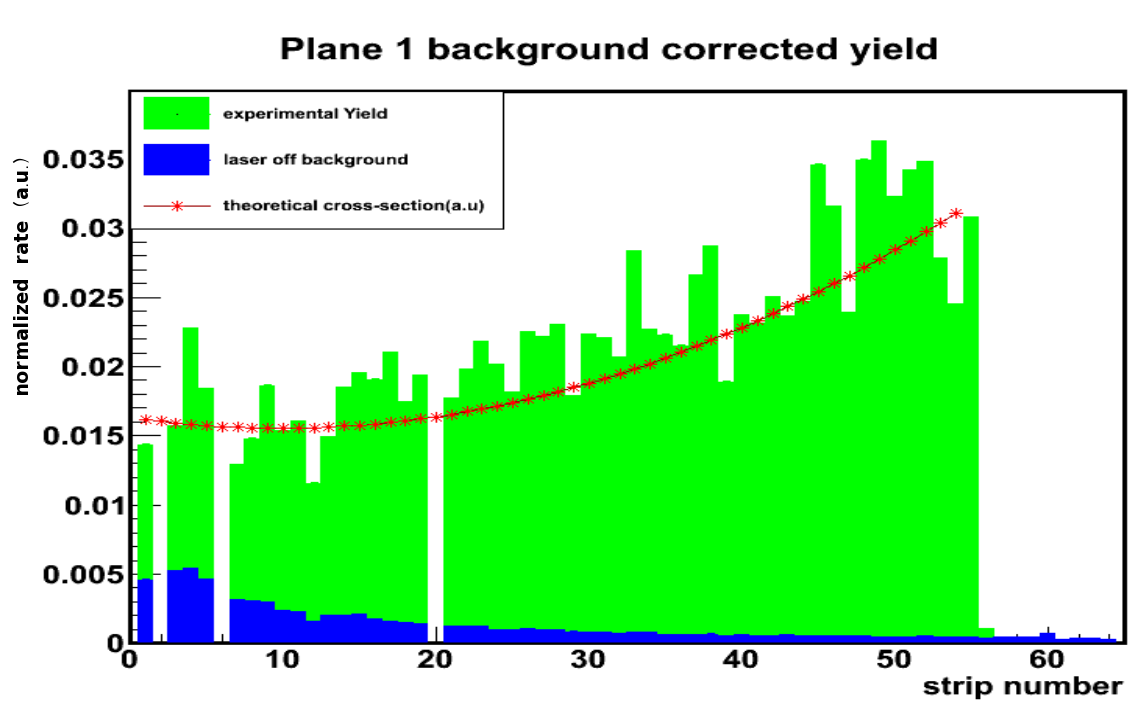
\includegraphics[width=0.6\textwidth]{Pictures/edet_spectrum.png}
\caption{Compton electron detector rate spectrum versus strip number (distance from electron beam). Blue is laser off background and green is background-subtracted laser on yield. Shape of theoretical Compton spectrum is shown by red curve.}
\label{fig:edet_spectrum}
\end{figure} 

Figure \ref{fig:edet_spectrum} shows the electron detector rate spectrum as a function of strip number or distance from electron beam. For the running conditions of \Q, the Compton edge was located $\sim$17~mm from the electron beam at the location of the electron detector. The electron detector was placed as close as 5~mm from the electron beam with the Compton edge around strip number 55.  Figure \ref{fig:edet_asym} shows a typical 1~hour asymmetry spectrum versus strip number. Variation in efficiencies from strip to strip create a jagged rate spectrum, but since the asymmetry is formed on a strip-by-strip basis, it is not affected  by efficiency to first order. Fitting the shape of the asymmetry spectrum maximizes the use of all the data and provides the highest precision measurement per unit time. During typical running conditions for Run 2 of \Q, the electron detector was able to reach a statistical precision of $\pm0.6\%$ in an hour.
\begin{figure}[ht]
\centering
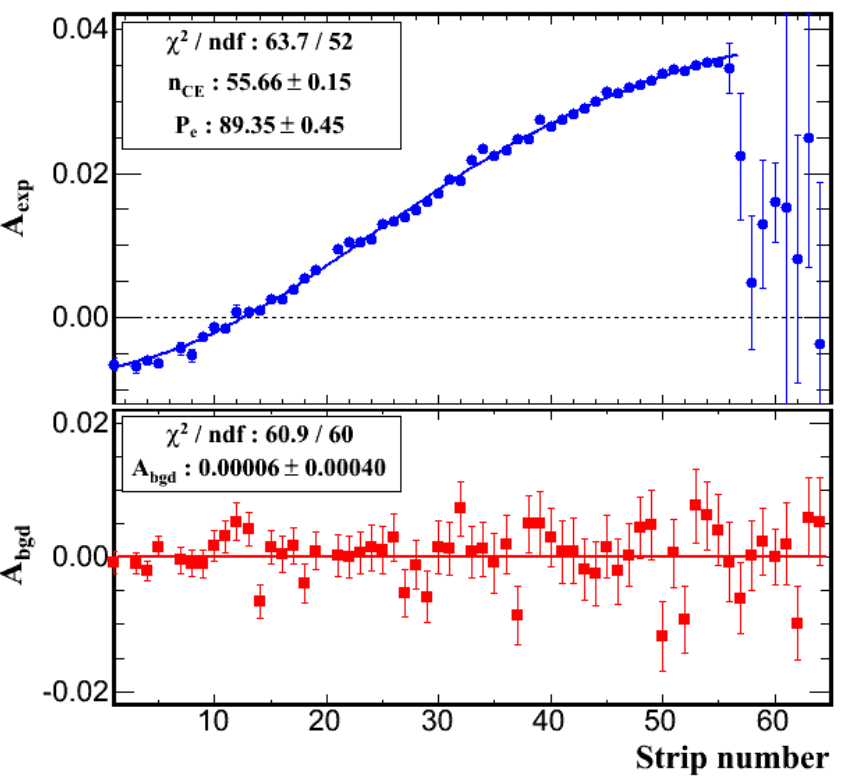
\includegraphics[width=0.6\textwidth]{Pictures/edet_asym.png}
\caption{Electron detector rate asymmetry versus strip number shown with fit to Compton spectrum with polarization of 89.4\%. Compton edge appears to be between strips 56 and 57. Background asymmetry is consistent with zero.}
\label{fig:edet_asym}
\end{figure} 

The quality of electron detector data was much higher in Run 2 than in Run 1 due to improvements made during the scheduled down time between the two run periods. During this down time the photon target power was doubled and the laser polarization increased. The electron detector pulse-conditioning electronics boards were replaced with improved, less noisy ones and a fourth electron detector plane was added. Analysis is ongoing to determine the electron detector polarizations and uncertainty for Run 1, while the Run 2 results are considered mature. A plot comparing the M\o ller and electron detector results for Run 2 is shown in Figure \ref{fig:Run2_edet_moller_pol}. A detailed account of the electron detector analysis can be found in \cite{Narayan}. Table \ref{tab:compton_systematics} lists the most significant contributions to the total systematic error for the Run 2 electron detector analysis.


\begin{figure}[ht]
\centering
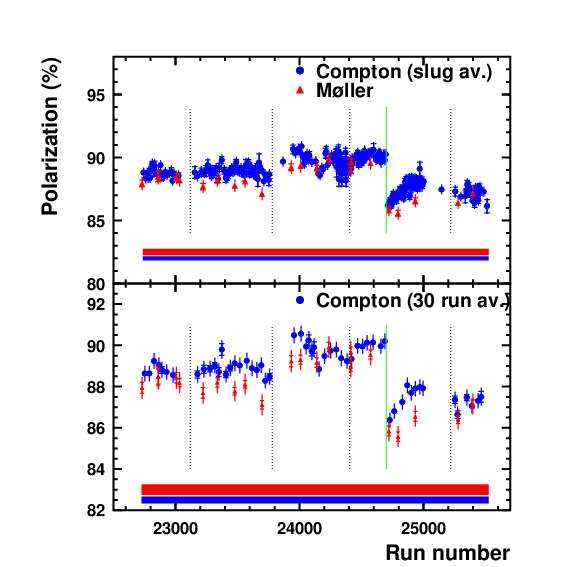
\includegraphics[width=0.6\textwidth]{Pictures/run2_moller_compton.png}
\caption{Electron beam polarization versus ``time'' results compared for M\o ller and Compton electron detector for Run 2 of \Q. Inner error bars are statistical and outer are systematic. Dashed vertical lines mark changes in position of electron source laser on the photo-cathode. Solid green vertical line marks heat and reactivation of source photo-cathode to increase quantum efficiency.   }
\label{fig:Run2_edet_moller_pol}
\end{figure} 

\begin{table}[ttbh]
%{\color{red}
\scriptsize{
  \centering
    \begin{tabular}{|l|c|c|} \hline
                            & Uncer- & $\Delta P/P$ \\ 
      Source 				& tainty & (\%) \\ \hline
      Laser polarization   		& 0.14 \%      & 0.14     \\
      Plane-to-plane  			& secondaries      & 0.00     \\
      3$^{rd}$ Dipole field		& 0.0011 T    & 0.13      \\
      Beam energy    			& 1 MeV   & 0.08     \\
      Detector $Z$ position      & 1 mm         & 0.03     \\
      Trigger multiplicity       & 1-3 plane         & 0.19     \\
      Trigger clustering         & 1-8 strips  & 0.01     \\
      Detector tilt ($X$)        & 1$^\circ$   & 0.03     \\
      Detector tilt ($Y$)        & 1$^\circ$   & 0.02     \\
      Detector tilt ($Z$)        & 1$^\circ$   & 0.04     \\
      Strip eff. variation        & 0.0 - 100\%   & 0.1     \\
      Detector Noise	         & $\leq$20\% of rate  & 0.1     \\
      Fringe Field		         & 100\%       & 0.05     \\
      Radiative corrections      & 20\%		   & 0.05     \\
      DAQ ineff. correction & 40\%  & 0.3     \\
      DAQ ineff. pt-to-pt	 & 		& 0.3     \\ 
      helicity correl. beam pos. & 5~nm & $<0.05$\\ 
      helicity correl. beam pos. & 5~nm & $<0.05$\\ 
      vert. pos. variation & 0.5~mrad & 0.2\\
      chicane spin precession    & 20~mrad & $<0.03$ \\ \hline
      Total                          &        & 0.58     \\ \hline
    \end{tabular}
  \caption{The Hall C Compton polarimeter systematic uncertainties determined for Run 2 of the experiment.}
  \label{tab:compton_systematics}
%  } %end color
}
\end{table}




\section{\label{sctn:target}Target}
The main production target for \Qs was a 34.4~cm long conical cell with thin aluminum windows, filled with \LHs and designed to handle the heat load introduced by a $180~\mu$A electron beam. A heat exchanger maintained the liquid hydrogen at 20~K and a variable-speed recirculating pump continually cycled the hydrogen through the target cell. The target cell was designed using Computational Fluid Dynamics, modeling fluid flow and heat load to mitigate the effects of target boiling, especially near target windows (see Figure \ref{fig:target_cell}). The target windows were made of a strong aluminum alloy Al 75075-T6 with the 22.2~mm diameter entrance window being 97~$\mu$m thick and the 305~mm diameter exit window having a thickness of 640~$\mu$m. Under nominal running conditions during \Qs the target heat load from ionization was 2.1~kW. The target heat exchanger was designed to accommodate 2.8~kW to allow for other sources of heating (such as the pump) and still leave a comfortable reserve of 250~W. 

\begin{figure}[ht]
\centering
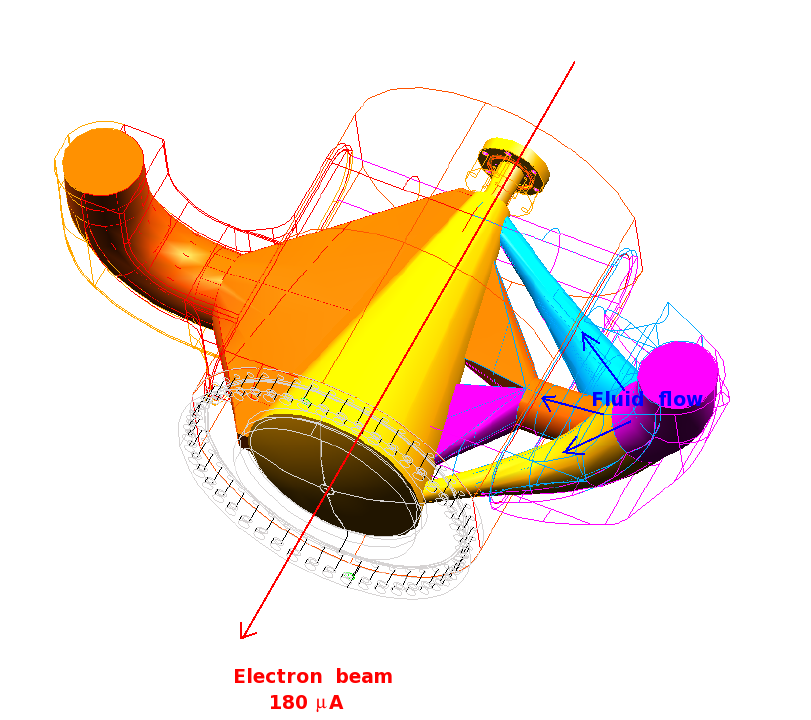
\includegraphics[width=0.6\textwidth]{Pictures/target_cell.png}
\caption{Rendering of the target cell with the exterior shell shown only in outline to expose the inner structure designed to optimize fluid flow for elimination of hot spots and minimal target boiling. The conical shape with a larger downstream window allowed all elastic events within the detector acceptance to pass without interference from other target cell structures.}
\label{fig:target_cell}
\end{figure} 

Target boiling is a source of excess width -- often called ``common-mode noise'' because it is seen by all the detectors -- in the main detector signal. One of the primary metrics used to evaluate the performance of the target was the additional width to the main detector asymmetry distribution attributed to target boiling. During production running the electron beam was rastered in a square pattern typically 4~mm~$\times$~4~mm to reduce target boiling and prevent burning the aluminum windows. A series of studies were done varying the target recirculation pump speed, the raster size and beam current to test the contribution to the main detector width from target boiling. Figure \ref{fig:boiling} shows the published results of one such test done by varying pump speed \cite{QweakNIM}. At the nominal \Qs production running conditions of 180~$\mu$A beam of 1.16~GeV electrons rastered in a square 4~mm~$\times$~4~mm pattern with a 28.5~Hz pump speed, the contribution to the main detector asymmetry width from target boiling was $53\pm5$~ppm, near the design limit of $<$50~ppm. 

\begin{figure}[hhbt]
\hspace*{0.75cm}
\centerline{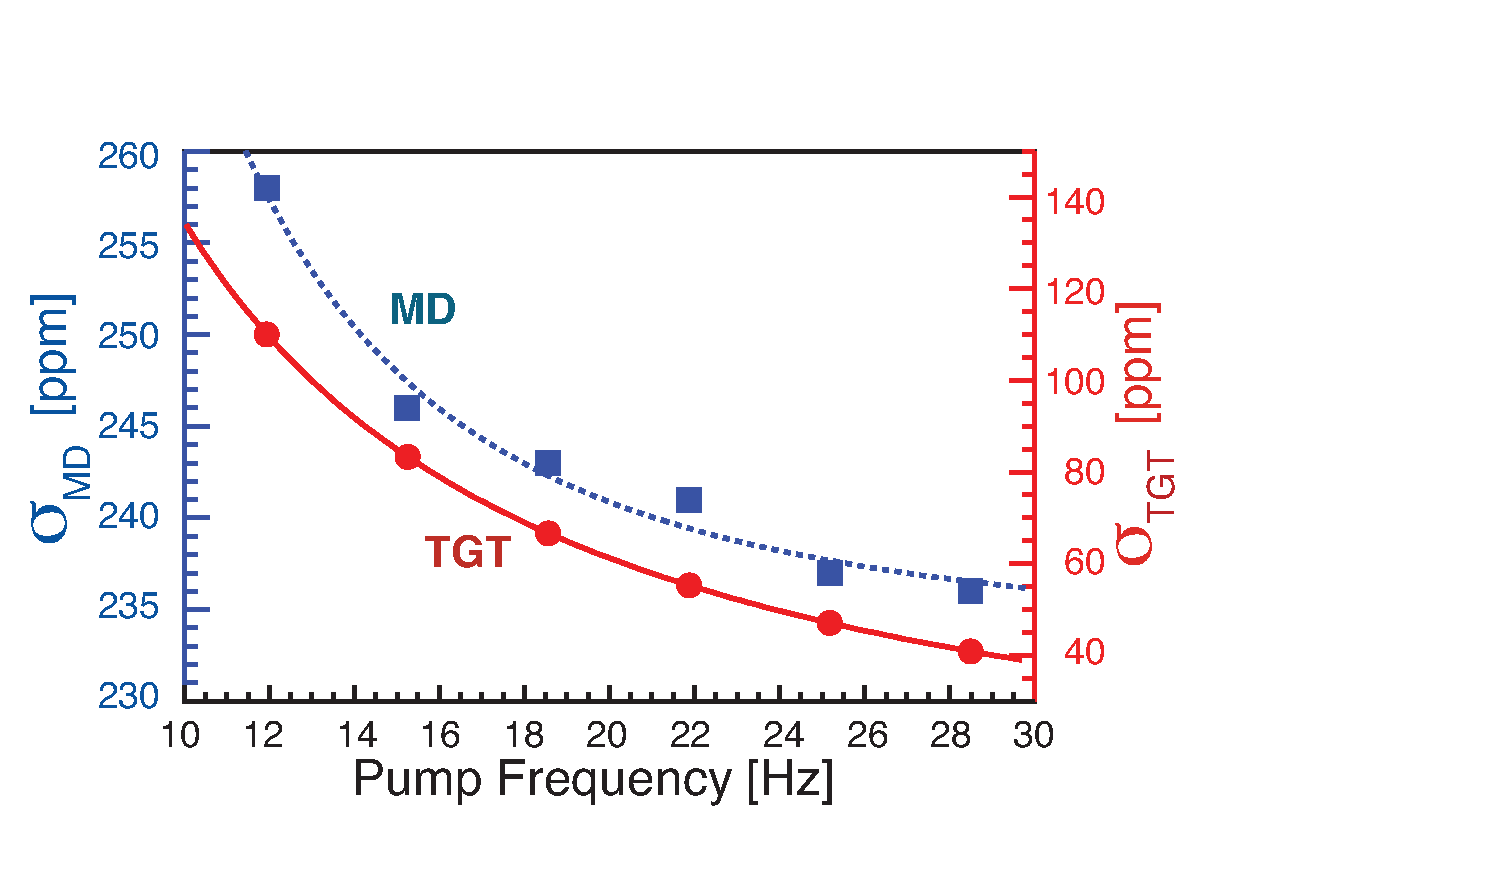
\includegraphics[width=0.75\textwidth,angle=0]{Pictures/pumpscan-eps-converted-to.pdf}}
\caption{\label{fig:boiling} Measured quartet-level main detector asymmetry width (solid blue squares) versus target recirculation pump rotational speed with 169~$\mu$A current and a 4$\times$4~mm$^2$ raster. Contribution to main detector width from target noise (red solid circles and right hand vertical scale), calculated under the assumption that the change in main detector asymmetry width comes solely from varying target noise (see \cite{Smith} for details on the study).}
\end{figure}

The target also included an array of solid targets on a ``ladder'' with locations along the beamline at the same position as the upstream and downstream aluminum windows. Aluminum solid targets of the same alloy as the target cell windows were used to measure the parity-violating asymmetry of aluminum  so that the window contribution could be removed from the main detector asymmetry measurement. Targets with various sizes of square holes were used to determine target alignment. Solid targets of carbon, beryllium and beryllium oxide were also included for possible systematic and calibration studies. A picture of the dummy target ladder in its September 2010 configuration is shown in Figure \ref{fig:dummy}. A few alterations to the targets were made between Runs 1 and 2 including the addition of more thin aluminum targets.

\begin{figure}[h]
\begin{minipage}{0.42\textwidth}
  \centering
  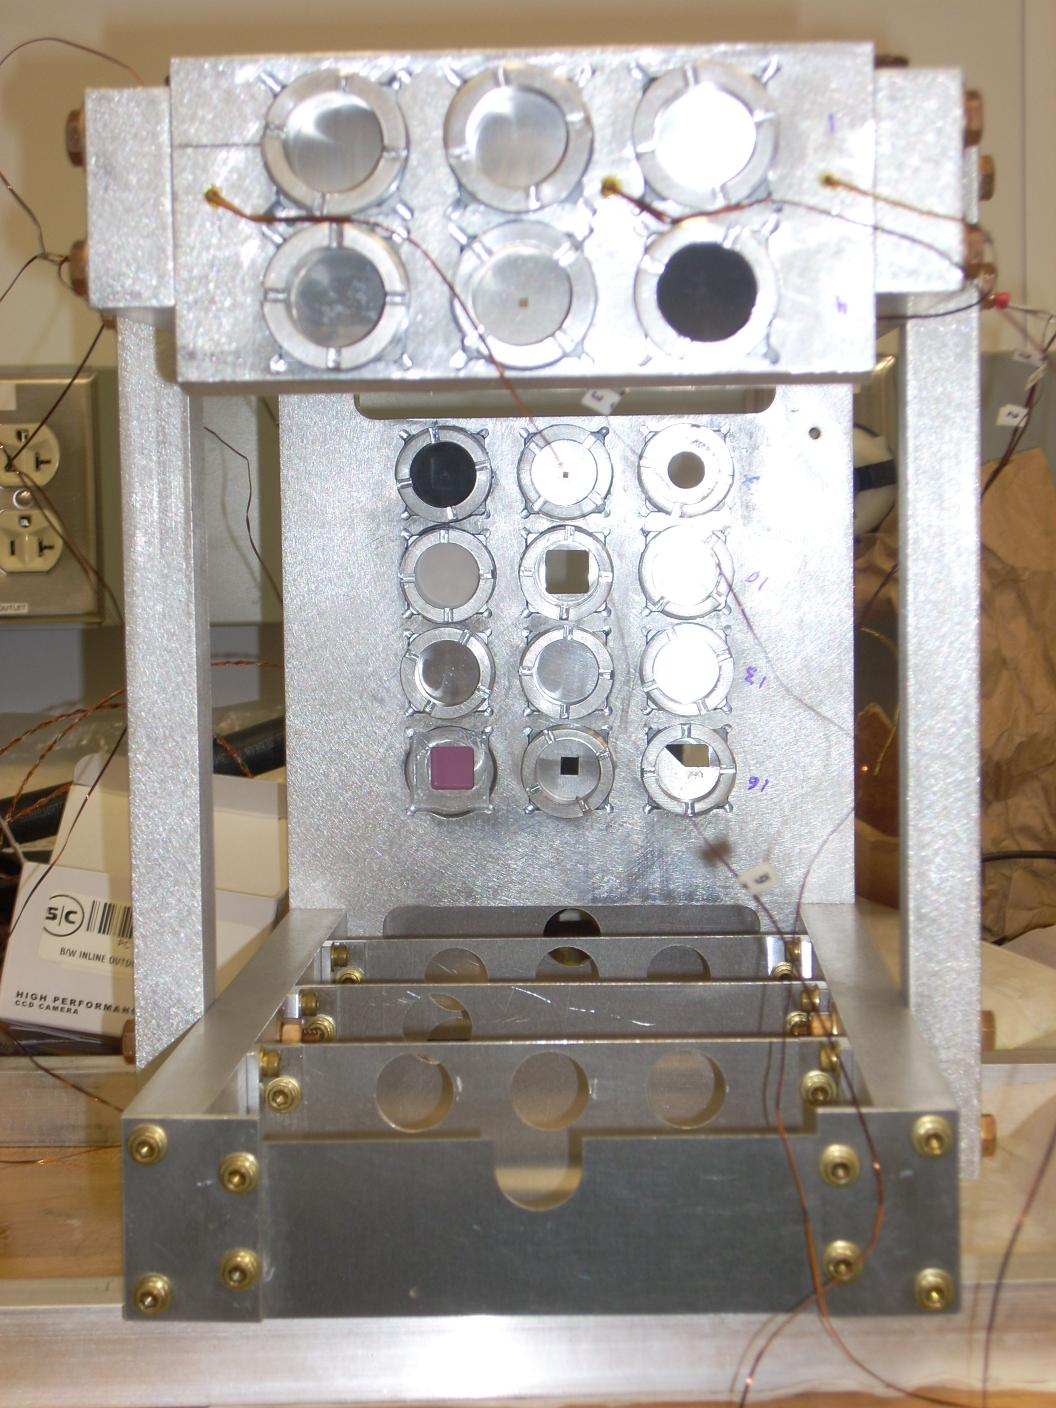
\includegraphics[width=0.9\textwidth]{Pictures/dummy_target.JPG}
\end{minipage}
\begin{minipage}{0.48\textwidth}
\centering
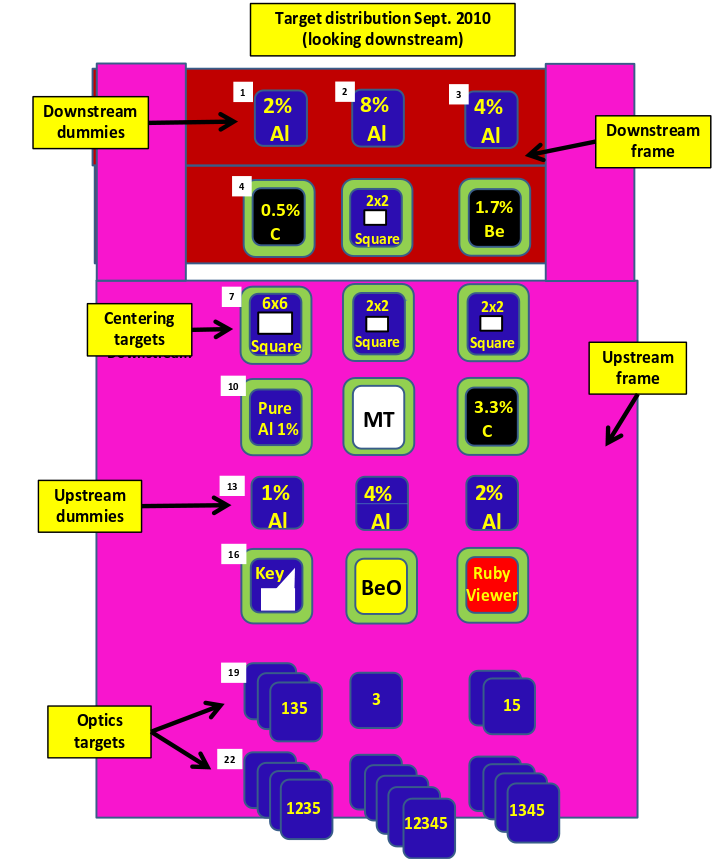
\includegraphics[width=1\textwidth]{Pictures/dummy_target_schematic.png}
\end{minipage}
\caption{\label{fig:dummy}Dummy target ladder for \Qs prior to Run 1. Picture on the left shows target ladder looking upstream. Schematic on right shows solid target configuration as it was before Run 1 looking downstream. Upstream and downstream targets of various materials were included. The most important solid targets were the aluminum targets at both upstream and downstream window locations used to measure the contribution of the aluminum target windows to the measured rates.}
\end{figure} 

\section{Collimation and Shielding}
Three lead collimators located between the target and spectrometer (see Figure \ref{fig:QweakApparatus}) formed the collimator system for the \Qs experiment. The first collimator located close to the target was a cleanup collimator used to reduce radiation for downstream equipment, whereas the second collimator defined the polar and azimuthal acceptance of the experiment. A third collimator located in the upstream fringe field of the spectrometer served to further reduce backgrounds before the spectrometer. Figure \ref{fig:collimators} shows the three main collimators during installation in Hall C. 
\begin{figure}[ht]
\centering
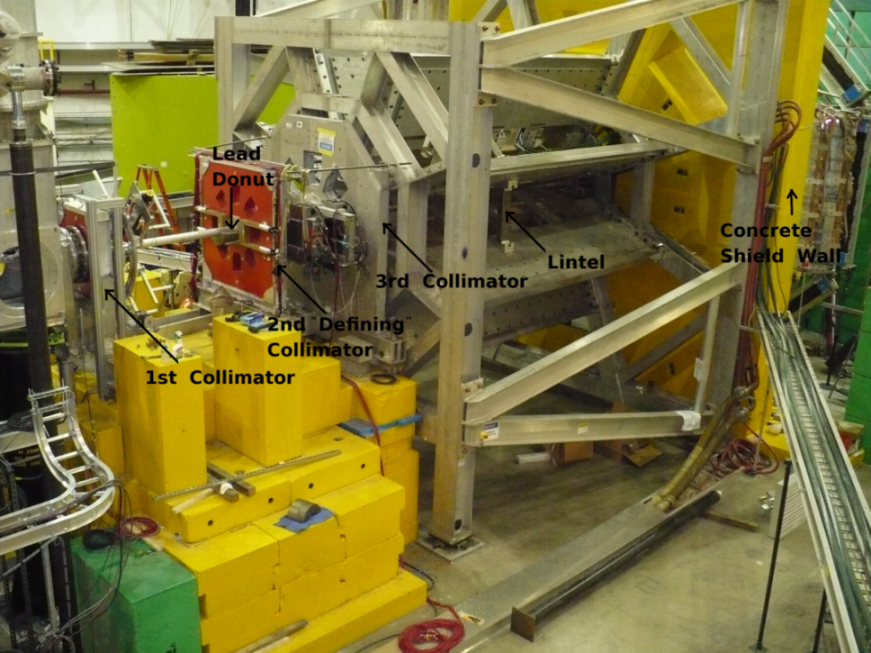
\includegraphics[width=0.8\textwidth]{Pictures/installed_collimators.png}
\caption{Picture showing the collimation system used in the \Qs experiment during installation in Hall C at Jefferson Lab. Also labeled are the lintels for blocking line-of-sight photons from the target and the lead donut around the beam pipe on the primary collimator which reduced backgrounds from beamline scattering.}
\label{fig:collimators}
\end{figure} 

A water-cooled, cylindrical tungsten collimator installed in the central aperture of the first collimator defined the maximum scattering angle that could pass through the beam enclosure and was designed to stop scattering with line-of-sight to the main detector. The tungsten collimator was machined to have a central conical shaped aperture with upstream and downstream diameters of 14.9~mm and 21.5~mm respectively. This collimator, located 47~cm downstream of the target exit window, was calculated to absorb a deposited power of 1.6~kW during typical production conditions. The tungsten collimator is associated with a significant source of helicity-correlated background seen uniformly by all the main detector bars and will figure prominently in discussions about beam corrections in following chapters. A picture of the tungsten collimator installed in the first collimator is shown in Figure \ref{fig:tungsten_plug}.
\begin{figure}[ht]
\centering
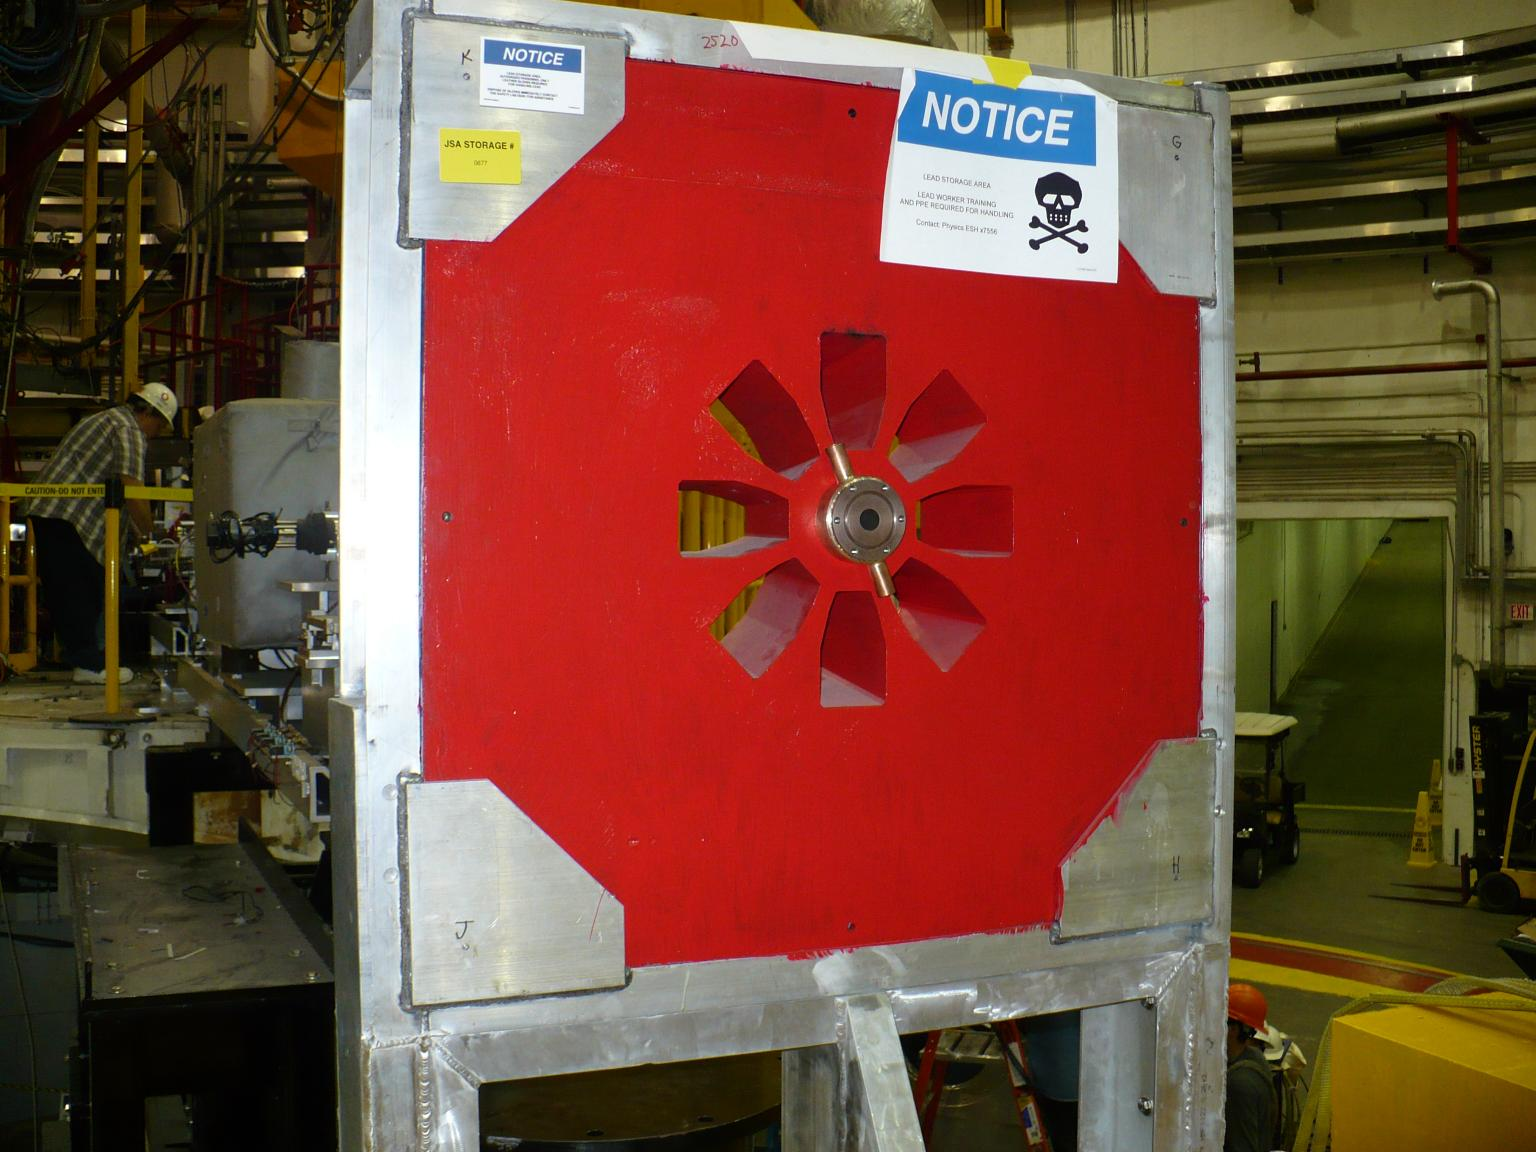
\includegraphics[width=0.6\textwidth]{Pictures/tungsten_plug.JPG}
\caption{First collimator shown with tungsten collimator installed in its central aperture. Perspective is looking upstream toward the target.}
\label{fig:tungsten_plug}
\end{figure} 

Lead ``lintels'' were installed inside the eight octants of the \qtor spectrometer to block line of sight photons to the main detector produced in the downstream edge of the defining collimator as well as in the tungsten collimator and the beam pipe just downstream of it. A lead donut was also installed around the beam pipe at the defining collimator (see Figure \ref{fig:collimators}) after it was determined to greatly reduce backgrounds in the main detector.

An 80~cm thick barite-loaded, stainless steel reinforced, high-density concrete wall was built just downstream of the detector to shield the main detector. The wall design was optimized using the GEANT3 simulation package to remove backgrounds associated with interactions of secondary photons and inelastic electrons in the main detector support structures. The apertures in this wall were designed to be well outside the elastic envelope defined by the second collimator and the \qtor optics.

During the scheduled accelerator down time between Runs 1 and 2, 5~cm thick insertable tungsten shutters were installed on the first collimator allowing octants 1 and 5 (octants located at 9 o'clock and 3 o'clock) to be completely blocked for dedicated background studies.  Further details of the shielding and collimation system and of the simulation efforts that went into their design can be found in \cite{Myers} as well as in the \Qs instrumentation publication \cite{QweakNIM}.

\section{\qtor Spectrometer}
The torroidal spectrometer (\qtor) employed in the \Qs experiment, in contrast to a pure momentum analyzing spectrometer, was designed to focus all elastic events inside the envelope defined by the collimator system into a mustache-shaped distribution on the detector bars. \qtor was composed of eight 3.7~m long, racetrack-shaped, double-pancake coils arranged symmetrically about a central axis to form eight octants. \qtor can be seen during installation in Figure \ref{fig:collimators}. The nature of \Qs required a highly degree of symmetry in the eight octants of the installed spectrometer. A precise mapping program that utilized shifts from predicted zero-crossings of the magnetic field in the fringe fields outside the ends of the spectrometer was used to determine coil misalignments. Details of this zero-crossing technique for determining coil misalignments are given in \cite{Wang}. The most important metric for quantifying design symmetry is the octant to octant variation of the total magnetic field seen by scattered electrons, often referred to as $\int B dl$. This variation was found to be within specified design tolerance of $\pm0.3\%$ (see page 28 \cite{QweakNIM}).

The \qtor spectrometer was composed of eight, water-cooled, resistive magnetic coils connected in series to a power supply. During nominal operating conditions \qtor ran at 8900~A and 123~VDC, generating a $\int B dl$ of 0.9~T-m at the mean scattering angle of $7.9^{\circ}$. Both the \qtor support structure and the coils were designed to be iron free to remove the possibility of helicity-correlated asymmetric scattering from magnetized iron reaching the detectors.

\section{Main Detector System}
The azimuthally symmetric main detector array for \Qs was designed to handle high rates with a high degree of linearity and low sensitivity to neutral backgrounds. The symmetric arrangement of the detectors also made their average response highly insensitive to shifts in beam position and angle. The main detector system comprised eight non-scintillating, quartz \v{C}erenkov bars, measuring 200~cm~$\times$~18~cm~$\times$~1.25~cm, arranged octagonally around the beam line at a radius of 335~cm. The quartz bars were sealed in light-tight enclosures and installed in a stiff aluminum support structure (see Figure \ref{fig:md_ferris}). The artificial fused-silica (Spectrosil 2000) bars were highly radiation hard and showed little yellowing over the course of the experiment even after sustaining a few thousand hours of rates as high as 900~MHz per bar. Figure \ref{fig:witness_plate} shows darkening of regular glass attached behind the main detector bars after only a few weeks of running. Each bar was composed of two 100~cm~$\times$~18~cm fused silica plates glued together in the center. An 18~cm~$\times$~18~cm~$\times$~1.25~cm waveguide glued to each end of the bar transported the light to 13~cm diameter PMT's which were glued to the downstream faces of the lightguides. 
\begin{figure}[ht]
\centering
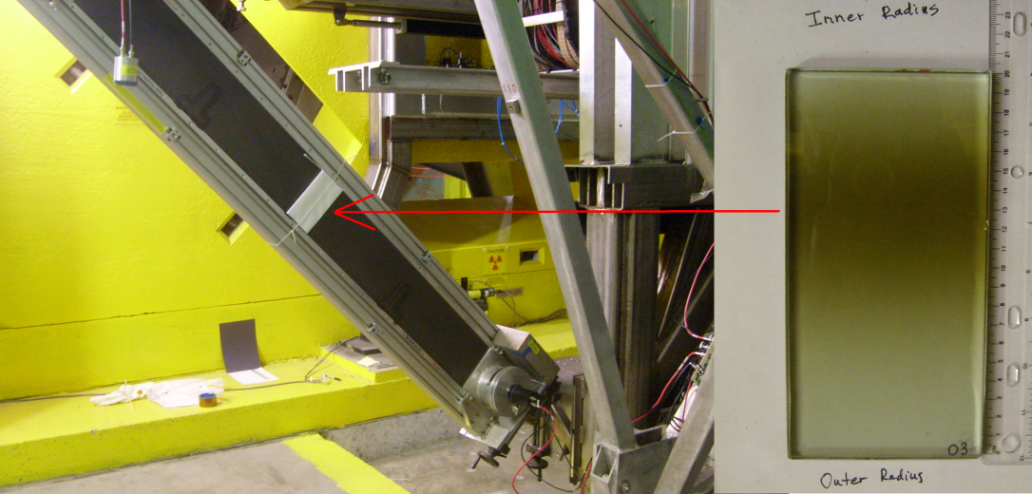
\includegraphics[width=0.8\textwidth]{Pictures/witness_plate.png}
\caption{Regular glass witness plates fastened to the downstream side of the main detector bar located and removed after only a few weeks of beam demonstrate clear darkening at the highest event region in the ``mustache'' distribution. Fused silica detector bars showed little radiation damage.}
\label{fig:witness_plate}
\end{figure}
\begin{figure}[ht]
\centering
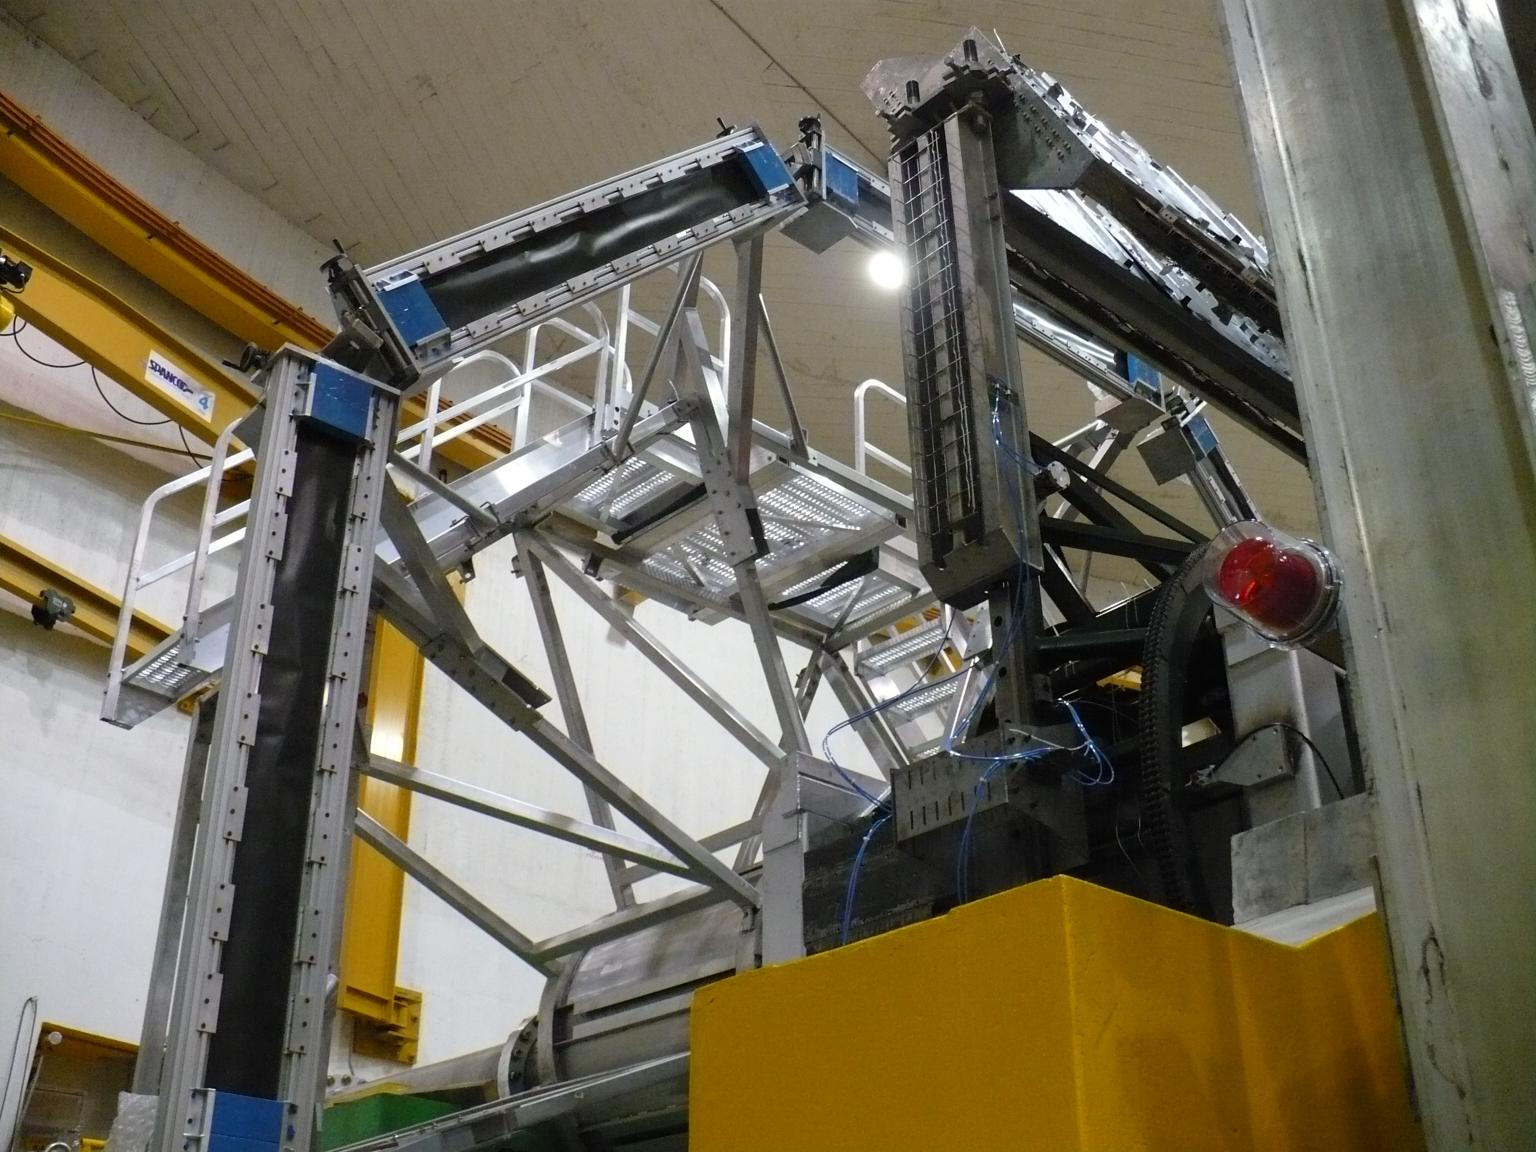
\includegraphics[width=0.8\textwidth]{Pictures/md.JPG}
\caption{Main detector bars seen during installation on the ``Ferris wheel'' support structure. Perspective is beam left looking downstream. Octants 1-3 are seen (see Figure \ref{fig:octant_coords} for explanation of coordinate terminology). Lead pre-radiators are not yet installed.}
\label{fig:md_ferris}
\end{figure}

A 2~cm thick lead pre-radiator was installed in front of each main detector bar to suppress low energy backgrounds. The pre-radiators increased light yield by a factor of 7 giving a signal to background improvement of 20 relative to test runs completed before the pre-radiators were installed. However, variation of shower size in the lead increased the main detector asymmetry width by 10\%. 

A bi-modal electronics readout chain allowed the main detector to operate in both high current (180~$\mu$A) and low current (50~pA) configurations. The high-current ``production mode'' for the experiment, designed for optimal accumulation of statistics, was an integrating configuration where each detector signal was digitally integrated and the average stored for each MPS. Low gain ($\sim10^3$) PMT bases with gain set close to 200, were used during high current running and the anode current was converted to voltage with a low noise, custom-made pre-amplifier. Low current or ``event mode'' was used with very low currents so that each event could be individually read out and the associated electron track from the target through the spectrometer could be reconstructed. Low current mode was used to check the alignment of the detectors and to verify simulated rates and event distributions on the bars. High gain ($\sim10^6$) PMT bases were installed for event mode running and individual pulses were digitized and stored. 

Digitization for the main detector signals (and many other diagnostic signals) was accomplished by custom built\footnote{Designed and built by TRIUMF in Vancouver, Canada.} 18-bit ADC's sampling at 500~kHz per channel.  

\begin{figure}[ht]
\centering
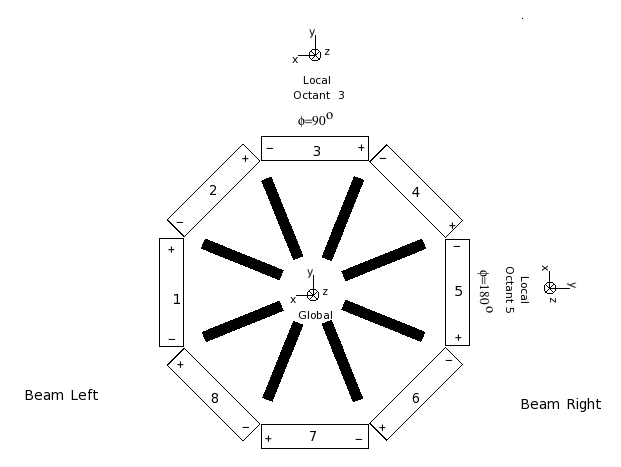
\includegraphics[width=0.6\textwidth]{Pictures/octant_coordinates.png}
\caption{Diagram of \Qs detector system looking downstream showing octant labeling. Numbered rectangles represent detector bars while solid spokes represent spectrometer coils.}
\label{fig:octant_coords}
\end{figure}

\section{Auxiliary Detectors}
A number of auxiliary detectors were added to the \Qs lineup to provide a variety of diagnostics. The main auxiliary detectors were the background detectors located inside the detector hut, a remotely controlled, movable focal plane scanner near main detector bar 7, upstream luminosity monitors (lumis) on the defining collimator and the downstream lumis 17~m downstream of the target. The design and use of each is discussed in the paragraphs ahead.
\begin{figure}[ht]
\centering
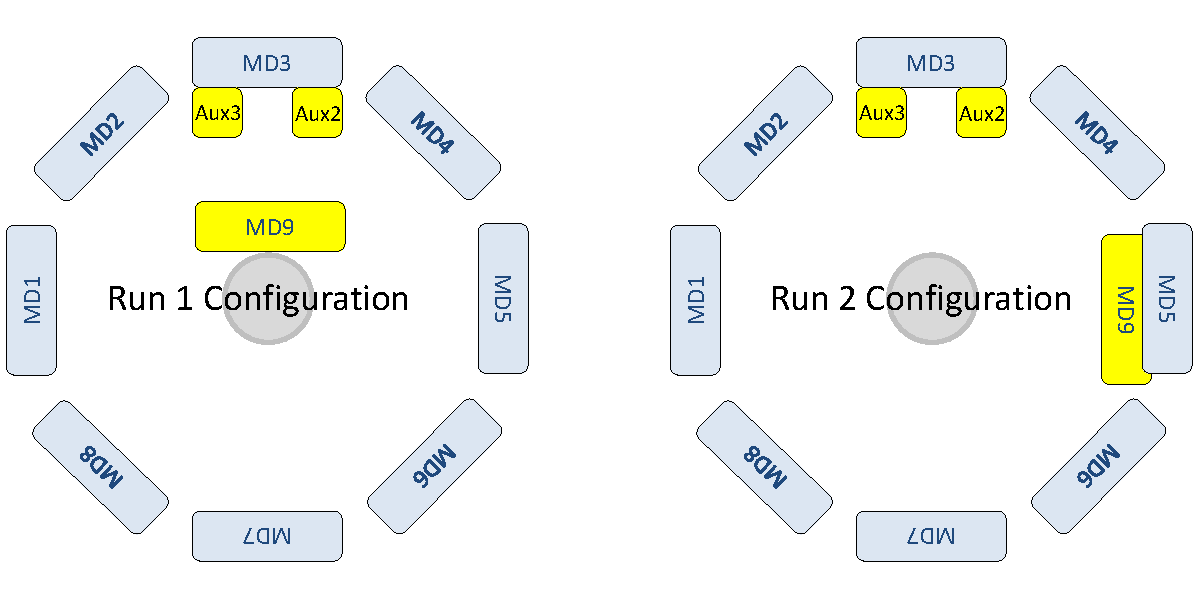
\includegraphics[width=0.7\textwidth]{Pictures/background_detectors.pdf}
\caption{Diagram showing the different positions of background detectors (yellow boxes) during Run 1 and Run 2. For a short period at the beginning of Run 1 the auxiliary detectors Aux2 and Aux3 were squeezed into the small spaces between detectors 5 and 6 and between detectors 1 and 8 respectively.}
\label{fig:background_det}
\end{figure}

\subsection{Background Detectors}
A set of detectors were installed inside the detector hut, outside the elastic envelope  to monitor backgrounds and to provide diagnostics for ruling out leakage of the helicity signal into the detector readout chain. The background detectors comprised a full \v Cerenkov detector bar assembly identical to the eight bars in the main detector array and three PMT's in dark boxes outfitted with LED light sources for testing, placed in various locations inside the detector shielding hut.

The background detectors were moved around during the early part of the \Qs experiment. Figure \ref{fig:background_det} summarizes the main configurations changes between Run~1 and Run~2. For the majority of the experiment (all of Run 2) the \v Cerenkov detector assembly called ``main detector 9'' or colloquially ``MD9'' since it was identical to the eight other main detector bars, was installed in the super-elastic region (smaller scattering angle than main detector acceptance) and slightly downstream of main detector bar 5 (MD5). The electronics and readout chain for MD9 were identical that of the main detector bars as well. Although MD9 was placed further into the super-elastic region than MD5 it also partially overlapped MD5 and derived part of its shower from events that passed through MD5, making its signal much more highly correlated with MD5 than with other main detector bars. 

The three ``dark box + PMT'' assemblies are referred to here as  Aux1-3. Aux1 remained near the floor in octant 7 and was illuminated with an LED to provide an anode current mimicking that of the main detectors during nominal production running. Aux1 is referred to colloquially as ``PMTLED''. PMTLED was fairly well shielded and was expected to have little response from scattering events. Its primary purpose was to verify that the main detector electronics chain was not picking up the helicity reversal signal. Aux2 was placed a meter downstream and on the super-elastic side of main detector 3 on beam right looking downstream, except for a short period at the beginning of Run 1 where it was installed in the gap between main detector bars 5 and 6. Aux2 was simply a PMT identical to the ones used on the main detector bars placed in a dark box and read out through the same signal chain as the main detectors. Aux2 was referred to colloquially as ``PMTONLY''. Aux3 was in the same position as Aux 2 except on beam left during most of the experiment with the exception of the same short period at the beginning of Run 1 when it was positioned in the space between main detector bars 1 and 8. It was composed of a PMT plus lightguide combination identical to those used in the main detector and was thus referred to as ``PMTLTG'' where ``LTG'' stands for ``lightguide''. Both PMTLTG and PMTONLY were used as background monitors for determining the background asymmetry contribution in the main detector. 

\begin{figure}[ht]
\centering
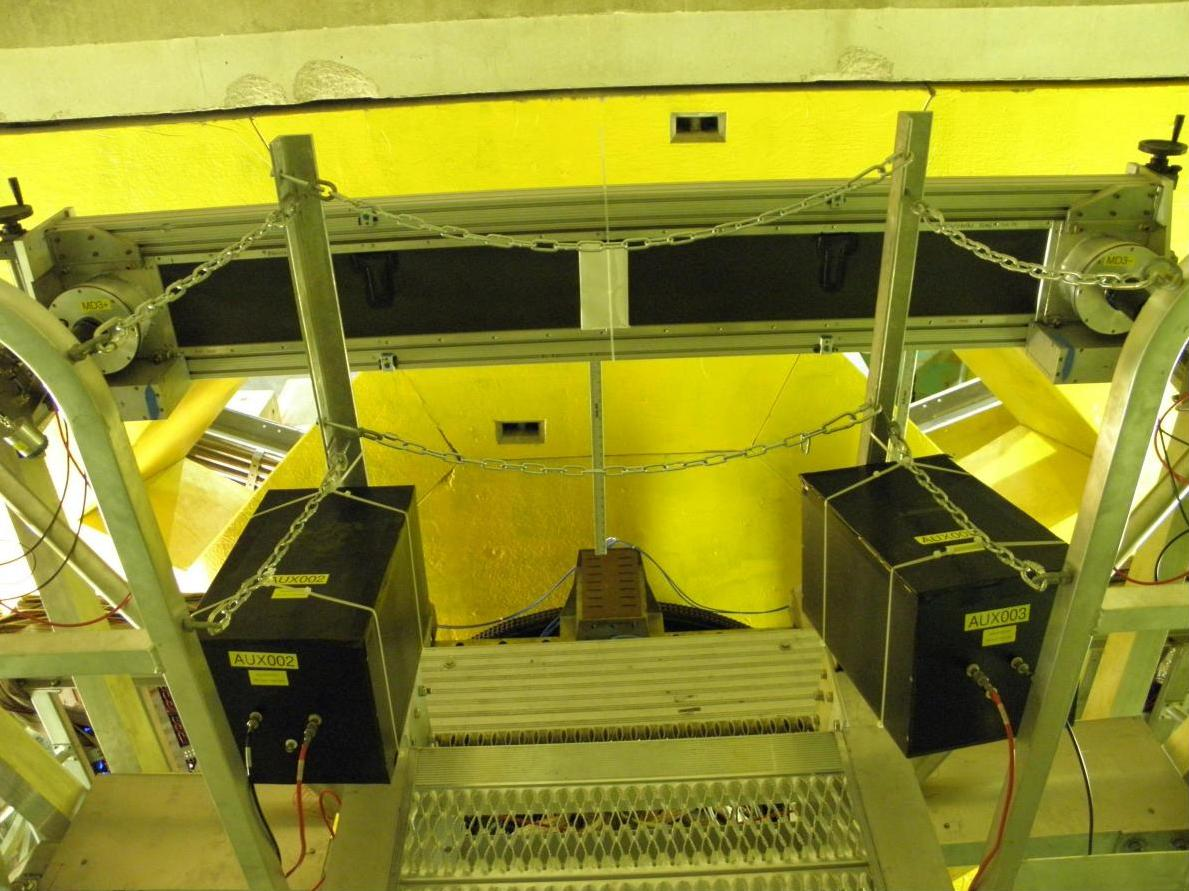
\includegraphics[width=0.6\textwidth]{Pictures/ltgandonl.JPG}
\caption{Picture showing Aux2 (PMTONLY) and Aux3 (PMTLTG) installed behind and below main detector bar 3.}
\label{fig:ltg_and_onl}
\end{figure}

\subsection{Focal Plane Scanner}
A focal plane scanner was used to map the distribution of events on MD7 and served as a diagnostic tool for verifying expected rate distributions from simulation. This scanner utilized two \v Cerenkov detectors each with a 1~cm$^3$ artificial fused silica crystal and installed to overlap so a single electron would create a pulse in both detectors. The quartz crystal were attached to waveguides and PMT's read out in coincidence. With a maximum main detector flux estimated to be 1~MHz/cm$^2$, the scanner was designed to be run in pulse counting mode even during high current running. The light guides were arranged in a V pattern to minimize accidental coincidences. Motion controllers with position read-back allowed the scanner to be rastered in a pre-set pattern over the face of MD7. The scanner could be installed to move across either the front or rear faces of the detector bar in order to map out the rate distributions. Figure \ref{fig:scanner} shows a picture of the scanner installed upstream of main detector bar 7 and a typical rate distribution from the hydrogen target.
\begin{figure}[h]
\begin{minipage}{0.45\textwidth}
\centering
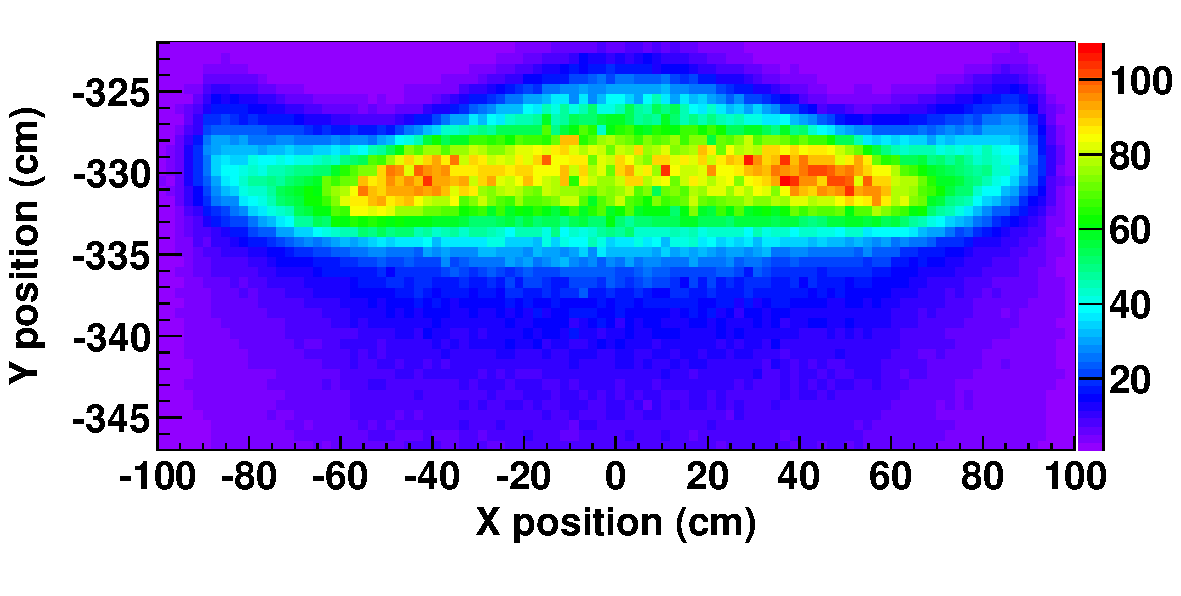
\includegraphics[width=0.98\textwidth]{Pictures/plot_ratemap.pdf}
\end{minipage}
\begin{minipage}{0.55\textwidth}
\centering
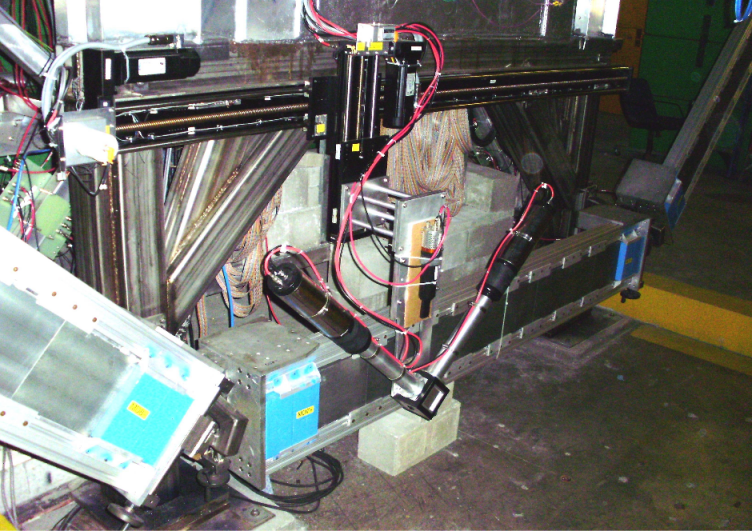
\includegraphics[width=0.98\textwidth]{Pictures/scanner.png}
\end{minipage}
\caption{(Left)Map of event distribution on detector bar 7 provided by the focal plan scanner showing ``mustache'' shape of elastic events focused by \qtor. (Right)Picture of the focal plane scanner shown installed in front of main detector bar~7. Two PMT and lightguide combinations were attached to overlapping fused silica crystals and the whole device could be scanned across the face of the detector bar to map out the distribution. A coincidence in both PMT's was required for an event to be recorded.}
\label{fig:scanner}
\end{figure}


\subsection{Upstream Luminosity Monitors}
The upstream luminosity monitors (upstream lumis), installed 1.76~m downstream of the target on the upstream face of the defining collimator (see Figure \ref{fig:uslumis}), were originally designed to measure target density fluctuations (boiling) and to provide immediate beam diagnostics. In the end, other methods utilizing scans of raster size and pump speed (see Section \ref{sctn:target}) were considered to be effective at determining the effects of target boiling. The upstream lumis, positioned close to the beam line, were designed to measure low angle ($\sim 5^{\circ}$) scatterers (primarily Mott and M\o ller) in the target and were required to withstand much higher rates than the main detectors. By extrapolation from low current running they were determined to receive 115~GHz at nominal production current of 180~$\mu$A. 

The upstream lumis were composed of a 25~cm~$\times$ 7~cm~$\times$ 2~cm strip of Spectrosil 2000 fused silica connected to 35~cm, air-filled, reflective aluminum light guides on each end. The light guides were continuously flushed with nitrogen to prevent degradation of the aluminum reflective surfaces from moisture or contamination. A 5.1~cm Hamamatsu PMT, attached to each light guide, was coupled to a bi-modal electronics readout chain designed to run in either current or event mode similar to the main detector. In current mode, unity-gain PMT bases were attached to voltage pre-amplifiers providing a DC signal that was then digitally integrated by the same TRIUMF ADC modules used for the main detector. In event mode, medium-gain PMT bases were coupled to fast pre-amplifiers read out by scalers for individual pulse counting. In low-current/event-mode, the upstream lumi count rates were scaled to estimate beam currents well below the useful limit of the BCM's. 

Correlations between the upstream lumis and the main detector and background detectors provided evidence that a key background seen in the main detector originated in the tungsten collimator. The upstream lumis which turned out to receive a large component of their signal from the tungsten collimator were a critical tool in the diagnosis and removal of this unwanted background component\footnote{A detailed analysis of the removal of this background is expected in a future thesis \cite{Kargiantoulakis}.}. 
\begin{figure}[ht]
\centering
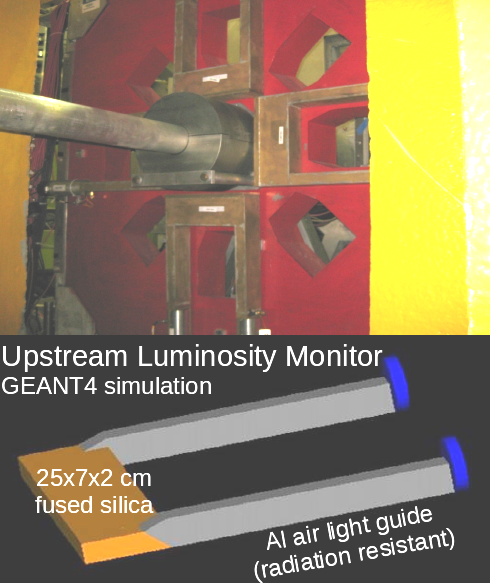
\includegraphics[width=0.5\textwidth]{Pictures/uslumis.png}
\caption{Picture of four upstream lumis installed on the upstream face of the defining collimator. The lower section of the figure shows a GEANT4 generated drawing of the upstream lumi construction.}
\label{fig:uslumis}
\end{figure}

\subsection{Downstream Luminosity Monitors}
The eight downstream luminosity monitors (downstream lumis) were installed 17~m downstream of the target (see Figure \ref{fig:dslumis}) in an azimuthally symmetric pattern around the beamline. They were originally designed to be a measure of the main detector null asymmetry and to provide immediate beam diagnostics. The downstream lumis, which penetrated the beam enclosure, were designed to measure low angle ($\sim 0.5^{\circ}$) scatterers (about equally sensitive to Mott and M\o ller events) in the target. Their proximity to the electron beam combined with the tight acceptance of the tungsten collimator prevented the downstream lumis from sampling scattering events in the region near the upstream target window. Their sensitivity to beam position made the downstream lumis useful monitors of beam position after the target. They received rates of 150~GHz at nominal production current of 180~$\mu$A.

The eight downstream lumis were each composed of a 4~cm~$\times$ 3~cm~$\times$ 1.3~cm strip of Spectrosil 2000 fused silica connected to a single 35~cm, reflective, nitrogen-flushed, aluminum light guide. Like the upstream lumis, PMT's attached to each light guide were coupled to a bi-modal electronics readout chain designed to run in either high current or event mode. Further details of the design and operation of both the downstream and upstream luminosity monitors can be found in \cite{Leacock2012}. 

\begin{figure}[ht]
\centering
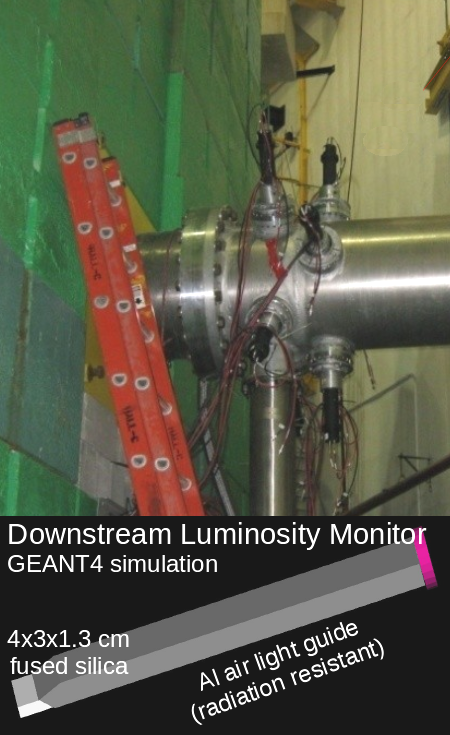
\includegraphics[width=0.5\textwidth]{Pictures/dslumis.png}
\caption{Picture of the eight downstream lumis installed downstream of the main detector array. The lower section of the figure shows a GEANT4 rendering of the downstream lumi construction.}
\label{fig:dslumis}
\end{figure}


\section{Tracking System}
The tracking system for \Qs was a set of detectors designed to provide track reconstruction for individual scattered electrons from their scattering vertex in the target to the main detector bars. The tracking system was used to characterized the main detector and map out its response, compare with/verify simulation and to reconstruct the average $Q^2$ and scattering angle of the experiment. It was divided into three regions. Region I between collimators 1 and 2 was intended to house a gas electron multiplier (GEM) detector for use in accurate vertex reconstruction but it was never operational during the experiment. Region II, located between the defining and 3rd collimators, housed a pair of horizontal drift chambers (HDC's) for vertex reconstruction and determination of scattering angle. Region III, located downstream of the spectrometer in the shielded detector hut near the focal plane, housed the vertical drift chambers (VDC's) that were used to accurately determine particle position and angle on the detector bars. Also in Region III were a set of trigger scintillators used during event mode to trigger events that would hit the detector bars.

For elastic ep scattering, simple relativistic kinematics neglecting the electron mass and radiative effects, relates the incoming electron energy $E$ to the outgoing scattered electron energy $E^{\prime}$ in terms of the lab frame scattering angle $\theta$ and the proton mass $m_p$ as
\begin{equation}
E^{\prime} = \frac{E}{1+2\frac{E}{m_p}\sin^2\frac{\theta}{2}}.
\label{eq:Eprime}
\end{equation}
The four momentum transferred from the electron to the proton is given by
\begin{equation}
  Q^2=\frac{4E^2\sin^2\frac{\theta}{2}}{1+2\frac{E}{m_p}\sin^2\frac{\theta}{2}}.
\label{eq:Qsquared}
\end{equation}

From this equation it appears that the only information required from the tracking system to completely determine the $Q^2$, is the scattering angle $\theta$ since the beam energy is known accurately from dedicated energy measurements described in Section \ref{sctn:btandm}. However, $\theta$ must be accurately acceptance-averaged and corrections must be applied for radiative effects in the target both before and after scattering requiring that the final $\langle Q^2 \rangle$ for the experiment be derived from simulation. The tracking system measurements are used to verify that the simulation is both correct and well understood. 

Both the HDC's and the VDC's are multi-wire, drift chambers designed to reconstruct a 3-dimensional electron trajectory. A plane of taut, evenly spaced sensing wires are kept near zero potential in a uniform electric field produced by a cathode held at a large negative potential. The entire chamber is flushed with a gas mixture chosen, among other characteristics, for its ionizability. An electron passing through the chamber creates a track of positive ions and electrons which then migrate along the electric field lines with the electrons accelerating towards the sensing wires. The strong electric fields near the wires accelerate the low energy ionization electrons to the point where they ionize other gaseous atoms causing a shower of as many as $10^6$ electrons. A pulse of measurable size is produced by the shower on the sensing wire. Readout is triggered by a set of plastic scintillators sensitive only to charged particles located near the detector focal plane. Time-to-digital converters (TDC's) were used to measure the time delay between the trigger and the pulse arrival on a given wire. Known drift times for the chambers provide the needed temporal-to-spatial conversions.   

The terms ``horizontal'' and ``vertical'' are derived historically from their typical orientations in previous experiments and are not descriptive of their orientations during the \Qs experiment. There are a few distinguishing features between HDC's and VDC's. HDC's are designed such that the ions drift parallel to the wire planes whereas the ions drift nearly perpendicular to the wires planes in a VDC. VDC's are typically designed to have the incident electron angle near $45^{\circ}$ whereas HDC's are installed such that the incident electron track is nearly normal to the wire plane. Also, drift times in HDC's are typically shorter allowing higher incidence rates. 

The HDC's used in \Qs were designed to have a large angular acceptance and to receive high rates since they were located in Region II before the spectrometer swept away the M\o ller events. During nominal running conditions in \Q, M\o ller rates in Region II were expected to exceed the ep scattering rates by a factor of 500. The HDC's consisted of two sets of drift chamber pairs each with an active area of 28~cm $\times$ 38~cm, and were located symmetrically on each side of the beam. The entire assembly of 4 drift chambers was attached to a mechanism designed to rotate by $\pm90^{\circ}$ to measure all octants. On either side of the beamline were two identical drift chamber assemblies with the second located 42~cm downstream from the first to provide angular resolution. Each drift chamber had 6 wire planes XUVX$^{\prime}$U$^{\prime}$V$^{\prime}$, with the wires in U and V at $\pm53.1^{\circ}$  relative to X. Measured position resolution for each chamber was in the 150-200~$\mu$m range giving an angular resolution of 0.6~mrad. A picture of the HDC's installed in Region II is shown in Figure \ref{fig:HDCs}.
\begin{figure}[ht]
%\begin{minipage}{0.6\textwidth}
\centering
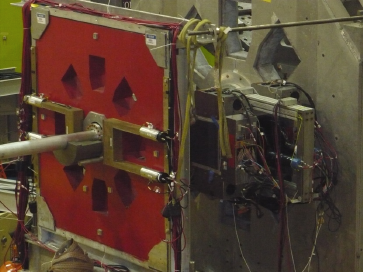
\includegraphics{Pictures/HDCs.png}
\caption{Picture of HDC's during installation in Region II. In this orientation the HDC's would measure tracks in octants 1 and 5.}
\label{fig:HDCs}
\end{figure}

The VDC's also consisted of two pairs or ``packages'' of drift chambers arranged symmetrically on opposite sides of the beamline fixed to a mechanism which allowed $\pm90^{\circ}$ rotation. The arms of the rotator also allowed for two radial positions, a retracted position close to the beamline for high current mode when the drift chambers were not being used and an extended position near the front of the main detector bars. A drawing of the rotator mechanism can be seen in Figure \ref{fig:VDC_rotator}. Each package has two drift chambers located 53~cm apart in the beam direction.

\begin{figure}[ht]
\centering
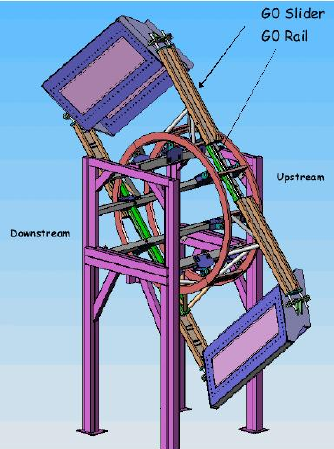
\includegraphics[width=0.5\textwidth]{Pictures/VDC_rotator.png}
\caption{Drawing of VDC's on rotator mechanism.}
\label{fig:VDC_rotator}
\end{figure}

Each of the four VDC drift chambers housed two wire planes with the wires strung at $\pm26.6^{\circ}$ relative to the long axis of the chambers. The active area of each chamber was 53.3~cm~$\times$~204.5~cm. A typical electron track at $45^{\circ}$ to the chamber triggered 6 wires in a given plane (see Figure \ref{fig:VDC_track} for illustration) with a maximum of 8 wires at the largest possible angle accepted. The position resolution of a single wire was in the 265-295~$\mu$m range. Using a separation of 53~cm between the two chambers in a given package and an average of 12 hits per chamber gives a naive angular resolution of about 0.15~mrad.
\begin{figure}[ht]
\centering
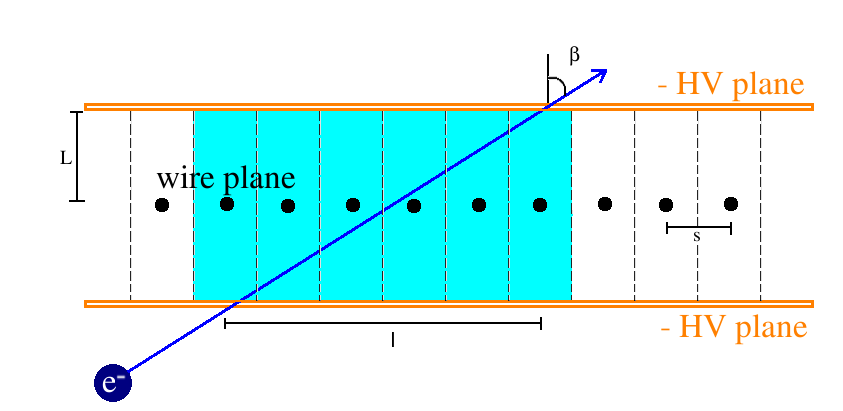
\includegraphics[width=0.8\textwidth]{Pictures/electron_track.png}
\caption{Illustration of electron track intersecting a single wire plane. L, s, l and $\beta$ are parameters used in the tracking analysis. }
\label{fig:VDC_track}
\end{figure}

The 2232 wires in the VDC's were read out using a custom-made multiplexing electronics readout which allowed sequential readout of multiple wires giving a factor nine fewer total TDC channels needed. Further details about the VDC's and track reconstruction can be found in \cite{Leckey2012}.

Track reconstruction was performed with an offline analysis using track pattern recognition algorithms. Straight line trajectories upstream and downstream of the spectrometer obtained from the HDC's and VDC's respectively, were crudely matched to each other using the known spectrometer field and an initial guess for the scattered electron energy $E^{\prime}$.  The guess for  $E^{\prime}$ was iteratively improved until the trajectories converged.
\begin{figure}[ht]
\centering
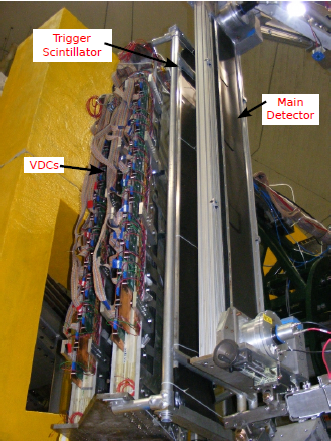
\includegraphics{Pictures/vdcs.png}
\caption{Picture of VDC's installed in Region III looking upstream towards spectrometer.}
\label{fig:vdcs}
\end{figure}
